\documentclass[a4paper,12pt]{article}
\usepackage{natbib}
\usepackage[english,ngerman]{babel}
\usepackage[utf8]{inputenc}
\usepackage[T1]{fontenc}
\usepackage{amsmath}
\usepackage{fullpage}
\usepackage{graphicx}
\usepackage{float}
\usepackage{booktabs}
\usepackage{prettyref}
\usepackage[a4paper,top=20mm]{geometry}
\usepackage{subfigure}
\usepackage{csquotes}
\usepackage{url}
\usepackage{array} % für bessere Tabellenkontrolle
\usepackage[export]{adjustbox}

\usepackage{longtable,booktabs}

\usepackage[table]{xcolor} % Farbe für Tabelle
\usepackage{siunitx} % SI-Einheiten
\sisetup{
  locale = DE,       % Dezimaltrennzeichen Komma (optional)
  detect-all         % benutzt Schriftart des Umgebungstextes
}


% Glossar
\usepackage[acronym,nonumberlist]{glossaries}
\makeglossaries

\newglossaryentry{flettner}{
  name={Flettner-Rotor},
  description={rotierender Zylinder, der mithilfe des Magnus-Effekts Vortrieb erzeugt}
}
\newglossaryentry{magnus}{
  name={Magnus-Effekt},
  description={seitliche Kraft auf einen rotierenden Körper im Strömungsfeld}
}
\newglossaryentry{debouncing}{
  name={Entprellen},
  description={Software- oder Hardware-Verfahren, um Prellimpulse mechanischer Schalter herauszufiltern}
}
\newglossaryentry{failsafe}{
  name={Failsafe},
  description={Sicherheitsfunktion, die bei Funkausfall Servo und ESC auf Neutral stellt}
}
\newacronym{esp32}{ESP32}{Mikrocontroller mit integriertem Wi-Fi und Bluetooth}
\newacronym{espnow}{ESP-NOW}{Peer-to-Peer-Funkprotokoll von Espressif}
\newacronym{adc}{ADC}{Analog-Digital-Wandler}
\newacronym{pwm}{PWM}{Pulsweiten-Modulation}
\newacronym{i2c}{I\textsuperscript{2}C}{Zweidraht-Bus}
\newacronym{isr}{ISR}{Interrupt Service Routine}
\newacronym{esc}{ESC}{Electronic Speed Controller}
\newacronym{bldc}{BLDC}{Brushless-DC-Motor}
\newacronym{bec}{BEC}{Battery Eliminator Circuit}
\newacronym{kv}{KV}{Drehzahlkonstante eines Motors in \(\mathrm{rpm/V}\)}
\newacronym{lipo}{Li-Po}{Lithium-Polymer-Akku}
\newacronym{fdm}{FDM}{Fused Deposition Modeling – Schmelzschichtverfahren}
\newacronym{cad}{CAD}{Computer Aided Design}
\newacronym{pla}{PLA}{Polylactid-Filament für 3D-Druck}
\newacronym{petg}{PETG}{Polyethylenterephthalat Glykol – zähes 3D-Druck-Filament}
\newacronym{tpu}{TPU}{Thermoplastisches Polyurethan – flexibles Filament}
\newacronym{asa}{ASA CF}{Acrylnitril-Styrol-Acrylat mit Carbonfasern}
\newacronym{ams}{AMS}{Automatic Material System von Bambu Lab}
\newacronym{rfid}{RFID}{Radio Frequency Identification – Funkchip}
\newacronym{ble}{BLE}{Bluetooth Low Energy}
\newacronym{lora}{LoRa}{Long Range Low-Power Funk}
% End of glossar


 
 % for code snippets
\usepackage{xcolor}
\usepackage{listings}

\lstdefinestyle{cppstyle}{
  language=C++,
  basicstyle=\ttfamily\footnotesize,
  numbers=left,
  numberstyle=\tiny,
  stepnumber=1,
  numbersep=5pt,
  showstringspaces=false,
  breaklines=true,
  backgroundcolor=\color{gray!5},
  keywordstyle=\color{blue}\bfseries,
  commentstyle=\color{green!60!black}\itshape,
  stringstyle=\color{orange}
}
\lstset{
  style=cppstyle,
  captionpos=b     % <-- caption at bottom
}

\renewcommand{\lstlistingname}{Quellcode}
% end of code snippets


\geometry{a4paper, margin=1in}
\pagenumbering{gobble}

\setlength{\parindent}{0pt}

\usepackage[colorlinks=true, linkcolor=blue, urlcolor=blue, citecolor=blue]{hyperref}

%================================================================
% Beginn

\begin{document}

% Bulme Logo eingebaut
\title{
  Diplomarbeit\\
  Flettner Aero Sail\\[1cm]
  \includegraphics[width=0.4\textwidth]{images/Bulme_Logo_blau.jpg}
}


%\title{Diplomarbeit\\Flettner Aero Sail}
\author{Kramperger Stefan\footnote{stefan.kramperger@gmail.com} \\ 
Meissl Alexander\footnote{alexander.meissl@bulme.at} \\
7/8ABELI}
\date{\today}
\maketitle
\newpage

\pagenumbering{Roman} % startet die romanische Nummerierung
\setcounter{page}{1}

\section*{Kurzbeschreibung}
\label{sec:Kurzbeschreibung}

% Um was geht es in der Arbeit
% Kramperger
Diese Diplomarbeit behandelt die Konstruktion, Entwicklung und Umsetzung eines Modellbootes, das mithilfe eines \gls{flettner}s angetrieben wird. Der Flettner-Rotor nutzt den Magnus-Effekt, um durch die anströmende Windkraft Vortrieb zu erzeugen. Im Zentrum des Projekts steht die vollständige Eigenentwicklung des Bootsaufbaus, der Steuerung und der dazugehörigen Software.\newline

Zu Beginn des Projekts wurde ein einfacher Versuchsaufbau realisiert, um grundlegende physikalische Eigenschaften des Flettner-Rotors unter kontrollierten Bedingungen zu untersuchen. Hierbei kamen verschiedene Windgeschwindigkeiten zum Einsatz, die mittels eines Turmventilators erzeugt wurden. Die gemessenen Effekte wurden auf einem karrierten Papier festgehalten und gaben Aufschluss über die Wirkungsweise des Rotors. Diese bildeten die Grundlage für das weitere Design. \newline

Basierend auf diesen Erkenntnissen wurde das Boot eigenständig modelliert und anschließend im 3D-Druckverfahren hergestellt. Als Bootsform wurde ein Katamaran gewählt, da dieser eine hohe Stabilität, geringen Tiefgang sowie optimale Voraussetzungen für die Platzierung und Ausrichtung des Rotors bietet. Die Konstruktion wurde in Fusion 360 entworfen, wobei Inspirationen aus bestehenden Konzepten, unter anderem aus Onlinequellen, einflossen. Besonderer Wert wurde auf ein modernes und funktionales Design gelegt.\newline

Parallel zur mechanischen Umsetzung entstand ein individuell entwickelter Controller, ebenfalls vollständig konstruiert und im 3D-Druckverfahren hergestellt, der eine feinfühlige Steuerung des Bootes ermöglicht. In mehreren Softwareentwicklungsphasen wurden die Funktionen der Steuerung schrittweise realisiert und kontinuierlich getestet. Diese iterative Herangehensweise erlaubte es, die Systeme stetig zu verbessern und sowohl die Effizienz als auch die Sicherheit des gesamten Aufbaus zu optimieren.\newline

Abschließend wurde das fertige Boot in einem selbstgebauten Becken getestet. Dieses Becken wurde aus Holzpfeilern und einer ausgekleideten Plane gefertigt und mit Wasser gefüllt. Durch sorgfältige Dokumentation der Testläufe konnten aussagekräftige Ergebnisse gewonnen werden, die die Funktionalität und das Potenzial des entwickelten Systems bestätigen. Die Arbeit zeigt die Machbarkeit und die vielseitigen Einsatzmöglichkeiten eines Flettner-Rotor-basierten Antriebskonzepts im Modellmaßstab auf und legt die Grundlage für weitere Optimierungen und Entwicklungen in diesem Bereich.

\newpage

\section*{Abstract}
\label{sec:Abstract}
This thesis focuses on the design, development, and implementation of a model boat powered by a Flettner rotor. The Flettner rotor utilizes the Magnus effect to generate propulsion by converting the force of oncoming wind into forward motion. At the core of the project is the complete in-house development of the boat's structure, its control system, and the associated software.\newline

At the beginning of the project, a simple experimental setup was realized to investigate the basic physical properties of the Flettner rotor under controlled conditions. Different wind speeds, generated using a tower fan, were directed at the rotor. The effects measured on a checkered sheet provided valuable insights into the rotor's behavior and formed the foundation for further design decisions.\newline

Based on these findings, the boat was independently modeled and subsequently manufactured using 3D printing. A catamaran hull was chosen due to its high stability, shallow draft, and optimal conditions for the placement and adjustment of the rotor. The construction was designed using Fusion 360, incorporating inspirations from existing concepts, including online sources. Special emphasis was placed on achieving a modern and functional design.\newline

In parallel with the mechanical construction, a custom-designed controller was developed, also fully created in Fusion 360 and manufactured via 3D printing, to provide a control solution tailored precisely to the project's needs. In several phases of software development, the control functionalities were progressively implemented and continuously tested. This iterative approach allowed for ongoing improvements to the system’s efficiency and safety.\newline

Finally, the completed boat was tested in a self-constructed pool. The pool was built from wooden beams and lined with a waterproof tarp, then filled with water and stabilized with additional weights. Careful documentation of the test runs using cameras, notes, and observations enabled precise analysis of the results. The work demonstrates the feasibility and the wide range of application possibilities of a Flettner-rotor-based propulsion concept on a model scale and lays the groundwork for future optimizations and developments in this field.

\newpage

\section*{Eidesstatliche Erklärung}
\label{sec:EidesstatlicheErklärung}

Die Verfasser erklären an Eides statt, dass sie die vorliegende Diplomarbeit selbstständig und ohne fremde Hilfe verfasst, andere als die angegebenen Quellen und Hilfsmittel nicht benutzt und die den benutzten Quellen wörtlich und inhaltlich entnommenen Stellen als solche kenntlich gemacht haben.\newline


\renewcommand{\arraystretch}{3} % 2 = doppelte Höhe
\begin{tabular}{|p{7.25cm}|p{0.5cm}|p{7.25cm}|}
    \hline
    Datum, Ort: & & Unterschrift: \\ \hline
    Datum, Ort: & & Unterschrift: \\ \hline
\end{tabular}

\newpage

\section*{Danksagung}
\label{sec:Danksagung}

Wir möchten uns an dieser Stelle herzlich bei unserem Betreuer Herrn DI DI Stephan Michelitsch für seinen engagierten Einsatz und seine Unterstützung während des gesamten Projekts bedanken.
Ein besonderer Dank gilt außerdem Herrn Dr. Roland Schmidt sowie Herrn DI Fritz Reissner von der Firma Geodata für ihre wertvolle Unterstützung im Projektverlauf.
Abschließend möchten wir uns auch bei Herrn DI(FH) Markus Kienreich für seine Unterstützung während der finalen Testphase bedanken.

\begin{table}[H]
\centering
\renewcommand{\arraystretch}{1.5}
\begin{tabular}{|p{5cm}|p{9cm}|}
\hline
\rowcolor{gray!30}
\textbf{Name des Diplomanden} & \textbf{Individuelle Schwerpunkte} \\
\hline
Meissl Alexander & 
\begin{tabular}[t]{@{}l@{}}
Planung und Montage \\
Konstruktion mit Fusion 360 \\
3D-Druck \\
Hardware-Implementierung und Verkabelung \\
Dokumentation
\end{tabular} \\
\hline
Kramperger Stefan & 
\begin{tabular}[t]{@{}l@{}}
Planung und Montage \\
Physikalische Berechnungen \\
Software-Implementierung \\
Dokumentation
\end{tabular} \\
\hline
\end{tabular}
%\caption{}
\label{tab:arbeitsschwerpunkte}
\end{table}

Die Verfasser der einzelnen Kapitel wurden wie folgt gekennzeichnet:

\begin{itemize}
    \item \texttt{[M]} – erstellt von Alexander Meissl
    \item \texttt{[K]} – erstellt von Stefan Kramperger
\end{itemize}


\newpage
\printglossary[type=\acronymtype,title={Abkürzungsverzeichnis}]
\printglossary[title={Glossar}]


\newpage
\tableofcontents
\newpage

\pagenumbering{arabic} % startet die arabische Nummerierung
\setcounter{page}{1} 


\newpage
%---------------------------------------------------------------------------------------------------
%---------------------------------------------------------------------------------------------------
% Kapitel 1
%---------------------------------------------------------------------------------------------------
%---------------------------------------------------------------------------------------------------
\section{Beschreibung der Theorie}
\label{sec:BeschreibungDerTheorie}

\subsection*{\texorpdfstring{Einleitung \textsubscript{[K]}}{Einleitung [K]}}
\label{sec:Einleitung}

Diese Diplomarbeit beschäftigt sich mit der Konstruktion und Umsetzung eines Modellbootes, das durch einen Flettner-Rotor\cite{wiki_flettner} angetrieben wird. Der Flettner-Rotor macht sich die physikalischen Eigenschaften des Magnus-Effekts\cite{wiki_magnus} zunutze, indem er die auf ihn wirkende Windkraft in einen Antrieb für das Boot umwandelt. Der Flettner-Rotor sitzt als eine Art drehbarer Zylinder auf dem Boot und nutzt die Form der Energieumwandlung für eine Vorwärtsbewegung. Die dafür notwendige Steuerung wurde über einen Controller realisiert, der diverse Steuerungselemente wie Joysticks und Drehimpulsgeber beinhaltet, um die Beschleunigung und Richtung des Bootes einfach steuern zu können. 
% Erster Versuchsaufbau
% Kramperger
Bevor das Boot in das erste Designstadium überging, mussten grundlegende physikalische Eigenschaften getestet werden, um eine grobe Einschätzung der Funktionalität zu bekommen. Es wurde ein prinzipiell einfacher Testaufbau gebaut, welcher die physikalischen Eigenschaften der Kraftentwicklung des Rotors in Abhängigkeit von der Windgeschwindigkeit und der Windrichtung emuliert. Mit einem Turmventilator sind 3 unterschiedliche Windstärken gezielt auf einen Rotor gelenkt worden und ein darunter liegendes karriertes Papier sorgte für eine 2-dimensionale Wertezuteilung. 
% Wie alles umgesetzt wurde
% Kramperger
Das Boot wurde selbst modelliert und 3D gedruckt, wobei Inspirationen von bestehenden Konstruktionen herangezogen wurden.
% Beschreibung der Konstruktion
% Meissl
\subsection*{\texorpdfstring{Beschreibung der Konstruktion \textsubscript{[M]}}{Beschreibung der Konstruktion [M]}}
\label{sec:Beschreibung der Konstruktion}
Die gesamte Konstruktion wurde mithilfe der \gls{cad}-Software Fusion 360 entworfen, anschließend im 3D-Druckverfahren hergestellt und zum Schluss manuell zusammengebaut. Als Bootsform wurde ein Katamaran gewählt, da dieser unter anderem eine hohe Stabilität, geringeren Tiefgang und optimal für die Platzierung und Einstellbarkeit des Rotors 
geeignet ist. Darüber hinaus diente auch ein YouTube-Video als Inspiration für die Wahl dieser Rumpfform. Diese Kombination aus fundierten Designüberlegungen und praktischer Inspiration ermöglichte eine effiziente Umsetzung des Projekts und veranschaulicht die vielfältigen Anwendungsmöglichkeiten moderner Konstruktions- und Fertigungsmethoden. Darüber hinaus spielte das Ziel, ein modernes Design umzusetzen, eine wesentliche Rolle bei der Gestaltung des gesamten Bootes.\cite{Website:Youtube}, \newline
Ein weiterer Punkt war die eigene Konstruktion und Umsetzung eines Controllers. Dieser wurde ebenfalls vollständig in Fusion 360 entwickelt und im 3D-Druckverfahren hergestellt, um eine auf das Projekt optimal abgestimmte Steuerungslösung zu erhalten.
% Versuche mit Software
% Kramperger
\subsection*{\texorpdfstring{Programmierung der Software \textsubscript{[K]}}{Programmierung der Software [K]}}
\label{sec:Programmierung der Software}
Parallel zur Konstruktion des Bootes wurden Programme geschrieben, die schrittweise die Funktionalität der Steuerung kreieren. Angefangen bei einfachen Programmen, die mit Lenken eines Joysticks den Antrieb des Motors steuern bis hin zu Programmen, welche die Kommunikation zwischen zwei Mikrocontrollern ermöglichen. Da die Implementierung immer nur schrittweise erfolgte, mussten hierfür auch viele Anpassungen und Tests durchgeführt werden, um möglichst viele unerwünschte Szenarien und Fehler auszubügeln. Das kontinuierliche Testen erlaubte das Einfügen vieler relevanter Features, welche nicht nur Effizienz, sondern auch Sicherheit bieten und somit ein wichtiger Bestandteil des ganzen Prozesses waren. 
% Test im Becken
% Kramperger
Der finale Testlauf wurde in einem selbstgebauten Becken durchgeführt. Dazu wurden Holzpfeiler miteinander verschraubt und mit einer Plane auslaufsicher ausgekleidet. Anschließend füllte man das Becken mit Wasser und stabilisierte es zusätzlich mit Gewichten. Der gesamte Versuch wurde dokumentiert.
\newpage

\subsection{\texorpdfstring{Die Physik hinter dem Magnus-Effekt und dem Flettner-Rotor \textsubscript{[M]}}{Die Physik hinter dem Magnus-Effekt und dem Flettner-Rotor [M]}}
\label{sec:Die Physik hinter dem Magnus-Effekt und dem Flettner-Rotor}
Das physikalische Prinzip des Flettner-Rotors beruht auf dem Magnus-Effekt. Gustav Magnus untersuchte dieses Phänomen erstmals um 1850. Er führte erste Versuche mit geometrischen Körpern durch, um deren Verhalten in Strömungen zu untersuchen. Dabei stellte Gustav Magnus fest, dass eine rotierende Kugel oder ein rotierender Zylinder eine seitlich wirkende Kraft erfährt. Diese Kraft lässt sich mithilfe der Bernoulli-Gleichung erklären.\cite{Flettner_Uni_Flensburg}\newline

Ein Flettner-Rotor nutzt genau dieses physikalische Prinzip, indem er als rotierender Zylinder in einem Luftstrom eine Querkraft erzeugt. Die Rotation des Zylinders führt dazu, dass die Strömungsgeschwindigkeit auf der einen Zylinderseite zunimmt (wenn sich die Zylinderoberfläche mit der Strömung bewegt), während sie auf der gegenüberliegenden Seite abnimmt (wenn sich die Oberfläche gegen die Strömung bewegt). Dadurch entsteht ein Druckunterschied um den Zylinder herum.

Die Bernoulli-Gleichung veranschaulicht diesen Effekt durch den Zusammenhang zwischen Strömungsgeschwindigkeit und statischem Druck. Anführend ist die Gleichung in der vereinfachten Form dargestellt. Dabei ist die Höhenlage als konstant anzunehmen.

\begin{equation}
p + \frac{1}{2} \rho v^2 = \text{konstant}
\end{equation}

Dabei ist:
\begin{itemize}
    \item $p$ der statische Druck,
    \item $\rho$ die Dichte der Luft,
    \item $v$ die Strömungsgeschwindigkeit.
\end{itemize}

Nach der Bernoulli-Gleichung gilt: Dort, wo die Strömungsgeschwindigkeit höher ist, ist der Druck entsprechend niedriger und umgekehrt. Der resultierende Druckunterschied erzeugt eine Kraft quer zur Strömungsrichtung: die sogenannte Magnus-Kraft.
Beim Flettner-Rotor nutzt man diese Kraft zur Erzeugung von Schub, beispielsweise auf modernen Schiffen zur Unterstützung des Antriebs.
Die Abbildung \ref{fig:Kräftedarstellung} zeigt die Strömung und die Kraft die bei einem Schiff mit Flettner Rotor wirken.\cite{Flettner_Rotor_Wiki}

\begin{figure}[H]
    \centering
    \includegraphics[width=0.4\linewidth]{Flettner_rotor_forces.svg.png}
    \caption{Kräftedarstellung \cite{Flettner_Rotor_Wiki}}
    \label{fig:Kräftedarstellung}
\end{figure}


%\begin{figure}[H]
 %   \centering
%    \includegraphics[width=0.5\linewidth]{Magnus_Effect_at_Flettner_Rotor_Boat.svg.png}
 %   \caption{Bild von: Von Dan-yell - Eigenes Werk, CC BY-SA 3.0}
  %  \label{fig:Flettner-Rotor}
%\end{figure}

\newpage


\subsection{\texorpdfstring{Boot-Aufbau (warum Katamaran, warum Flosse) \textsubscript{[M]}}{Boot-Aufbau (warum Katamaran, warum Flosse) [M]}}
\label{sec:Boot-Aufbau}

Bei der Art des Bootes fiel die Entscheidung auf einen Katamaran. Durch die Doppelrumpfbauweise ergibt sich eine hohe seitliche Stabilität, was besonders bei Wellengang oder bei einer ungleichmäßigen Gewichtsverteilung durch die Elektronik wichtig ist. Der Katamaran liegt sehr stabil im Wasser und kippt kaum zur Seite, was eine gleichmäßige Rotation des Rotors begünstigt.\newline

Die Katamaran-Bauform bietet optimale Voraussetzungen für die Installation des Rotors und der Elektronikbox. Der Motor und der Rotor werden über einen Riemen angetrieben. Da der Riemen für einen effizienten Antrieb optimal gespannt sein muss, ist die Bauform des Bootes ideal, da der Rotor und sein Halter sehr variabel einstellbar sind. Ein weiterer Grund, warum die Entscheidung auf einen Katamaran gefallen ist, liegt im geringeren Tiefgang im Vergleich zu anderen Bauformen. Auch der optische Aspekt spielte bei der Wahl des idealen Bootes eine Rolle.\newline

Die Konstruktion des Bootes wurde mit Fusion 360 umgesetzt und die Teile im 3D-Druckverfahren hergestellt. Als Drucker kam der BambuLab P1S zum Einsatz, der sich durch seine hohe Druckqualität und Genauigkeit für dieses Projekt besonders gut eignet.

Das Boot besteht aus zwei Rümpfen, auch Schwimmer genannt. Diese laufen zur Bugspitze hin spitz zu, um den Wasserwiderstand zu minimieren. Weitere Bestandteile sind eine Mittelplatte, die beide Rümpfe verbindet, eine Elektronikbox, eine Flosse, ein Rotorhalter sowie der Rotor selbst. Beim Rotor handelt es sich um einen Zylinder mit jeweils einer Scheibe an den Enden. Zur Richtungssteuerung wurde am Heck des Bootes ein Ruder installiert. Die Flosse ist an der Unterseite der Elektronikbox montiert. Sie ist essenziell, damit das Boot geradeaus fährt und nicht abdriftet.\newline


Platzierung der Flosse: Die Flosse wurde bewusst direkt unter der Elektronikbox positioniert, da sie den Schwerpunkt des Bootes zentral hält. Die Flosse wirkt wie eine feste Kielstruktur und sorgt dafür, dass das Boot bei Geradeausfahrt nicht ungewollt seitlich abdriftet - insbesondere bei Wind- oder Rotorbetrieb. Sie verbessert somit maßgeblich die Kursstabilität.\newline

Modularität und Wartung: Alle Komponenten sind modular aufgebaut und lassen sich einzeln austauschen. Die Elektronikbox kann beispielsweise leicht entnommen werden, um an der Verkabelung oder an der Software zu arbeiten. Auch der Rotor lässt sich schnell demontieren, was Reparaturen oder Upgrades erheblich vereinfacht.


Nach der Montage aller Bauteile wurden erste Testfahrten in einer Badewanne durchgeführt, um die Funktionalität der Mechanik und Elektronik zu überprüfen. Besonderes Augenmerk lag dabei auf dem Tiefgang sowie der Balance des Bootes. Durch das zusätzliche Gewicht des Akkus und der gesamten Peripherie erhöhte sich die Gesamtmasse des Bootes deutlich. Trotz dieser zusätzlichen Belastung zeigte sich die Konstruktion stabil und bewahrte eine gleichmäßige Wasserlage. Auch die Abdichtung der Elektronikbox konnte in diesem frühen Stadium erfolgreich getestet werden. Die Tests bestätigten, dass das Boot grundsätzlich seetauglich ist und eine gute Basis für weitere Optimierungen bietet.



\newpage
\subsection{\texorpdfstring{Antriebsarten und welcher Motor verwendet wurde \textsubscript{[M]}}{Antriebsarten und welcher Motor verwendet wurde [M]}}
\label{sec:Antriebsarten}

Als Antriebsmotor wurde der Brushless-DC-Motor Kyrio A2212 mit 2200 KV gewählt. Dieser Motor überzeugt durch seine kompakte Bauweise (Durchmesser: ca. 27 mm, Länge: ca. 30 mm) und sein geringes Gewicht von etwa 52 g, wodurch er sich besonders für leichte und platzsparende Anwendungen eignet. Mit einer maximalen Leistung von ca. 200-250 W bietet er ausreichend Antriebskraft für das geplante Einsatzszenario. Darüber hinaus ist der Motor gut kompatibel mit handelsüblichen elektronischen Drehzahlreglern (\gls{esc}s) sowie dem verwendeten \gls{esp32}-Mikrocontroller, was eine unkomplizierte Ansteuerung über \gls{pwm}-Signale ermöglicht.\cite{Brushless_DC}


            \subsubsection{Prinzip des Brushless Motors:}
            \label{sec:Prinzip des Brushless Motors}
            Ein Brushless DC-Motor (\gls{bldc}-Motor) ist ein elektrisch kommutierter Gleichstrommotor, der im Gegensatz zu klassischen DC-Motoren keine mechanischen Bürsten oder einen Kommutator verwendet. Stattdessen erfolgt die Kommutierung - also das Umschalten der Stromrichtung in den Motorwicklungen - elektronisch über eine externe Steuereinheit.

            \subsubsection{Aufbau:}
            \label{sec:Aufbau des Motors}
            Stator: Der unbewegliche Teil des Motors enthält die Wicklungen (Spulen), die das Magnetfeld erzeugen. Diese Wicklungen sind auf einer festen Struktur befestigt und werden durch die Steuerelektronik angesteuert.\newline
            Rotor:
            Der drehbare Teil des Motors trägt Permanentmagnete, die durch das sich ändernde Magnetfeld des Stators in Rotation versetzt werden.
            \subsubsection{Funktionsweise:}
            \label{sec:Funktionsweise des Motors}
            Das Grundprinzip beruht auf der Wechselwirkung zwischen dem magnetischen Feld des Stators und den Permanentmagneten des Rotors. Durch gezieltes Ansteuern der Spulen im Stator mit Gleichstrom - typischerweise über ein dreiphasiges System - wird ein rotierendes Magnetfeld erzeugt. Dieses zieht die Magnete des Rotors mit sich, wodurch eine gleichmäßige Drehbewegung entsteht.
            Die elektronische Kommutierung erfolgt mithilfe von Sensoren (z.B. Hallsensoren), welche die Position des Rotors erfassen. Alternativ kann auch eine sensorlose Kommutierung über die Rückspannung der Motorphasen erfolgen. Die Steuerungselektronik nutzt diese Information, um den Stromfluss in den Spulen zeitlich genau zu schalten.
            \subsubsection{Vorteile gegenüber bürstenbehafteten Motoren:}
            \label{sec:Vorteile gegenüber bürstenbehafteten Motoren}
            Wartungsfreiheit: Da keine Bürsten vorhanden sind, entfallen mechanischer Verschleiß und regelmäßiger Austausch.\newline
            Höhere Effizienz: Durch den Wegfall der Reibungsverluste an Bürsten-Kollektor-Systemen.\newline
            Geringere Geräuschentwicklung: Besonders vorteilhaft in Anwendungen mit hohen Anforderungen an Laufruhe.\newline
            Bessere Regelbarkeit: Die elektronische Steuerung ermöglicht präzise Drehzahl- und Positionsregelung.\newline


            \newpage
            


    
        \subsubsection{ESC (Electronic Speed Controller):}
        \label{sec:ESC}


Für das Projekt wurde ein bidirektionaler 40A-Elektromotorregler (ESC) ausgewählt. Dieser ist vollständig kompatibel mit einem 2S-\gls{lipo}-Akku (7,4V) und kann darüber hinaus Spannungen bis zu 6S (22,2V) verarbeiten. Dank der bidirektionalen Funktionalität ist es möglich, die Drehrichtung des angeschlossenen Motors elektronisch zu steuern - ein entscheidender Vorteil bei Anwendungen, die sowohl Vorwärts- als auch Rückwärtsbewegungen erfordern.\newline

In Kombination mit einem bürstenlosen Außenläufermotor vom Typ 2212 mit 2200\gls{kv} ermöglicht diese ESC eine präzise und schnelle Steuerung des Antriebssystems. Die Plug-and-Play-Ausführung des Reglers erfordert keine Kalibrierung des Gaswegs und erleichtert dadurch die Inbetriebnahme erheblich. Für den Betrieb muss der Gashebel beim Einschalten in Mittelstellung stehen, um ein unerwartetes Anlaufen des Motors zu vermeiden.\newline

\textbf{Technische Daten der ESC:}
\label{sec:Technische Daten der ESC}

- Dauerstrom: 40A\newline  
- Eingangsspannung: 2-6S LiPo (7,4-22,2V)\newline 
- \gls{bec}: 5V / 3A (integriert)\newline
- Betriebsmodi: Bidirektional (ohne Bremse), erlaubt sofortige Richtungsumkehr\newline  
- Steuersignal: Plug and Play, keine Kalibrierung erforderlich\newline
- Startbedingung: Gashebel muss beim Einschalten in Mittelstellung stehen\newline  
- Anwendungsbereiche: RC-Autos, Boote, Unterwasserantriebe (z.B.: Thruster)\newline  
- Abmessungen: ca. 130 × 89 × 9mm\newline  
- Gewicht: ca. 41g  \newline

Diese ESC eignet sich besonders gut für Projekte, bei denen eine kompakte Bauweise und eine zuverlässige Steuerung in beide Drehrichtungen erforderlich sind. Die Kombination mit dem 2200kV-Motor stellt dabei eine leistungsfähige und vielseitige Lösung für den Antrieb dar.




    
    \subsubsection{Servomotor:}
    \label{sec:Servomotor}
    Für die Ansteuerung des Ruders kommt ein digitaler Hochleistungsservo des Typs DS3218 der Firma Miuzei zum Einsatz. Dieser hat genug Leistung um das Ruder unter Wasser anzusteuern. Die digitalen Steuerungseigenschaften ermöglichen eine genaue Positionsregelung.\cite{Datenblatt_Servomotor}\newline

    Technische Eigenschaften: Der DS3218 ist ein digital gesteuerter RC-Servo, der bei einer Betriebsspannung von 6,8V ein maximales Haltemoment von 21,5 kg·cm erreicht. Die Stellgeschwindigkeit beträgt 0,14 s pro 60° bei dieser Spannung. Dies gewährleistet eine schnelle und kraftvolle Reaktion des Rudersystems - auch unter Lastbedingungen wie Seitenwind oder bei dynamischer Steuerung während der Fahrt.\cite{Datenblatt_Servomotor}\newline
    
    Anwendung im Projekt: Das Servo übernimmt die Funktion der aktiven Steuerung der Ruderflächen um das Boot präzise steuern zu können.
    
    

\newpage

\subsection{\texorpdfstring{Dimensionierung des Bootes und des Rotors \textsubscript{[M]}}{Dimensionierung des Bootes und des Rotors [M]}}
\label{sec:Dimensionierung des Bootes}
\subsubsection{Dimensionierung mit Bootslänge von 500 mm}

Die Länge des Bootes wurde auf 500 mm festgelegt, da sich dieses Maß optimal mit dem vorhandenen 3D-Drucker realisieren lässt. Für die Dimensionierung des Rotors wurde das Verhältnis zwischen Bootslänge und Rotorhöhe anhand bestehender und erfolgreich umgesetzter Projekte untersucht. In vielen dieser Projekte hat sich ein Verhältnis im Bereich von etwa 1:1,4 bis 1:1,6 als besonders geeignet erwiesen, da es eine gute Balance zwischen Stabilität und Effektivität des Flettner-Rotors ermöglicht.\cite{Flettner_Uni_Flensburg}\newline

Allerdings zeigte ein Vergleich mit realen Anwendungen sehr unterschiedliche Umsetzungen: So lag das Verhältnis bei der Buckau bei etwa 2,95:1, bei der Barbara bei 5,1:1, beim Frachtschiff E-Ship 1 bei 4,8:1 und beim Modellboot Uni-Kat Flensburg bei 1,5:1. Diese große Spannbreite verdeutlicht, dass die ideale Dimensionierung stark vom konkreten Einsatzszenario und den Rahmenbedingungen abhängt.

Für unser Projekt wurde nach Abwägung verschiedener technischer Faktoren ein Verhältnis von 1,9:1 gewählt - also etwas höher als in den zuvor genannten Modellprojekten. Dies resultierte in einer Rotorhöhe von 263 mm bei einer Bootslänge von 500 mm:

\[
\frac{500 \, \text{mm}}{1.9} = 263 \, \text{mm}
\]

Ausschlaggebend für die Wahl dieses leicht erhöhten Verhältnisses war vor allem die Anpassung an die vorhandene Führungsstange, die in ihrer Länge eine technische Obergrenze für die Rotorhöhe vorgab. Darüber hinaus spielte auch die angestrebte Stabilität des Gesamtsystems eine wesentliche Rolle. Der Rotor sollte groß genug sein, um eine spürbare Wirkung im Modellmaßstab zu erzielen, aber gleichzeitig kompakt genug, um mechanisch sicher und ruhig geführt werden zu können. So wurde eine Bauweise gefunden, die sich sowohl praktikabel fertigen lässt als auch im Betrieb zuverlässig und effizient funktioniert.

\subsubsection{Dimensionierung der Gesamtbreite des Bootes}

Die Breite des Katamarans wurde im Rahmen des Projekts auf 300 mm festgelegt. Ausschlaggebend für diese Entscheidung waren in erster Linie die baulichen Beschränkungen durch den 3D-Drucker, insbesondere hinsichtlich des verfügbaren Bauraums. Bei einer gewählten Bootslänge von 500 mm ergibt sich daraus ein Breiten-Längen-Verhältnis von:

\[
\frac{300\, \text{mm}}{500\, \text{mm}} = 0{,}6
\]

Das bedeutet, die Breite beträgt 60\% der Gesamtlänge des Bootes.

Zum Vergleich: Beim akademischen Projekt „Uni-Kat Flensburg“, das ebenfalls ein katamaranartiges Flettner-Rotor-Schiff im Modellmaßstab umsetzte, wurde bei einer Länge von 6,1 m eine Breite von 4,5 m realisiert. Daraus ergibt sich ein Verhältnis von etwa 0,74. Obwohl das eigene Modell geringfügig schmaler gebaut wurde, liegt der Wert in einem realistischen und praxisnahen Bereich. Die Wahl der Breite stellt einen Kompromiss zwischen Druckbarkeit, Stabilität und Platzbedarf für die Elektronik sowie den Rotor dar und hat sich in den Testläufen als funktional erwiesen.\cite{Flettner_Uni_Flensburg}

\newpage

\subsubsection{Berechnung des Rotordurchmesser}
\label{sec:Berechnung des Rotorsdurchmesser}
Die Dimensionierung des Rotordurchmessers wurde auf Basis eines Fachartikels der Fachhochschule Flensburg vorgenommen, in dem verschiedene Rotorgrößen realisierter Flettner-Systeme untersucht werden. Darin werden unter anderem zwei zentrale Ausführungen beschrieben: Ein Flettner-Rotor mit einer Höhe von 27 m und einem Durchmesser von 4 m (Verhältnis 6,75:1) sowie ein zweiter mit 15,6 m Höhe und 2,8 m Durchmesser (Verhältnis 5,57:1). Der Mittelwert dieser beiden Verhältnisse liegt bei etwa 6:1.\cite{Fachhochschule_Flensburg}\newline

Für das eigene Modell wurde jedoch bewusst ein kleineres Verhältnis von rund 4,3:1 gewählt. Hintergrund dieser Entscheidung war einerseits der Wunsch nach einem stabileren, mechanisch belastbaren Rotor und andererseits spezifische technische Anforderungen im Modellmaßstab. Bei einer festgelegten Rotorhöhe von 262,5 mm ergab sich daraus ein Rotordurchmesser von etwa 61 mm.\newline


\textbf{Die Formel zur Berechnung des Rotordurchmessers:}

\[
\frac{262.5 \, \text{m}}{61 \, \text{m}} = 4.30
\]\newline

Ein entscheidender Grund für den größeren Durchmesser war die Integration einer inneren Führung mit Kugellagern. Diese Konstruktion erhöht die Laufruhe und Stabilität des Rotors erheblich und reduziert mechanische Reibungsverluste. Der zusätzliche Bauraum im Inneren ermöglichte eine einfache Aufnahme der Lager, ohne die strukturelle Integrität oder das vorgesehene Design zu beeinträchtigen.

Zudem erleichtert der etwas größere Durchmesser die Montage und Befestigung an der Führungsstange, da dadurch mehr Platz für passgenaue Verbindungselemente zur Verfügung steht. Die Wandstärke des Rotors blieb dabei unverändert.\newline

Es wird davon ausgegangen, dass der leicht erhöhte Durchmesser im Modellmaßstab keine signifikanten aerodynamischen Nachteile mit sich bringt, da bestimmte Strömungseffekte in dieser Größenordnung nur eingeschränkt skalierbar sind.


\newpage

\subsection{\texorpdfstring{Filamente für 3D Druck und welcher Drucker wurde verwendet \textsubscript{[M]}}{Filamente für 3D Druck und welcher Drucker wurde verwendet [M]}}
\label{sec:Filamente für 3D-Druck}

Im Rahmen dieses Projekts kamen verschiedene Filamente von Bambu Lab zum Einsatz, die speziell für den Einsatz mit den hauseigenen 3D-Drucksystemen optimiert wurden. Die Kombination aus Drucker, AMS-System (Automatic Material System) und herstellereigenem Filament bietet zahlreiche Vorteile, insbesondere im Hinblick auf Effizienz, Zuverlässigkeit und Benutzerfreundlichkeit.

Ein wesentlicher technischer Vorteil besteht in der RFID-basierten Materialerkennung. Jedes Original-Filament von Bambu Lab ist mit einem RFID-Chip ausgestattet, der relevante Materialparameter wie Drucktemperatur, Flussrate oder Rückzugseinstellungen enthält. Beim Einlegen der Spule in das AMS-System werden diese Informationen automatisch erkannt und an den Drucker übermittelt. Dadurch entfallen manuelle Einstellungen und potenzielle Fehlerquellen beim Materialwechsel.

Das AMS-System selbst ermöglicht den parallelen Einsatz mehrerer Filamente und unterstützt automatische Materialwechsel - z.B. für mehrfarbige Drucke oder den nahtlosen Wechsel zwischen Haupt- und Stützmaterial. In Kombination mit den optimierten Filamentprofilen sorgt dies für konsistente Druckergebnisse, selbst bei komplexen Geometrien oder Materialwechseln während des Druckprozesses.

Darüber hinaus sind alle Bambu Lab Filamente auf wiederverwendbaren Spulen erhältlich, was den Materialabfall reduziert und zur Nachhaltigkeit des Gesamtsystems beiträgt.\newline

\subsubsection{3D Drucker Bambu Lab P1S}
\label{sec:Bambu Lab P1S}

Der Bambu Lab P1S ist ein leistungsstarker, benutzerfreundlicher \gls{fdm}-3D-Drucker (Fused Deposition Modeling, auf Deutsch auch: Schmelzschichtungsverfahren), der speziell für hohe Druckgeschwindigkeit, Präzision und Materialvielfalt ausgelegt ist. Er basiert auf dem bewährten CoreXY-Mechanismus und ist werkseitig vorkalibriert, was einen schnellen und unkomplizierten Einstieg in den Druckbetrieb ermöglicht.

Dank seines geschlossenen Bauraums ist der P1S besonders gut für das Drucken technischer Materialien wie ABS, \gls{asa} oder PC geeignet, da die konstante Umgebungstemperatur die Druckqualität verbessert und Verzug reduziert. Der Bauraum misst 256 × 256 × 256 mm, was für die meisten Anwendungen im Modellbau, funktionalen Prototyping oder Bildung ausreichend Platz bietet.

Der Drucker erreicht eine maximale Druckgeschwindigkeit von 500 mm/s, mit einer Beschleunigung von bis zu 20000 mm/s², was ihn deutlich schneller macht als viele klassische Desktop-Drucker. Die Düsentemperatur kann bis 300°C, das Heizbett bis 100°C betrieben werden. Damit ist er mit einer breiten Palette an Filamenten kompatibel - von Standardmaterialien wie \gls{pla} oder \gls{petg} bis hin zu technischen Werkstoffen wie PA, CF-Verstärkte Filamente oder \gls{tpu}.

Der P1S ist vollständig mit dem \gls{ams}-System (Automatic Material System) von Bambu Lab kompatibel. Dieses ermöglicht automatischen Mehrfachmaterialdruck, Materialwechsel und die Verwendung von \gls{rfid}-erkannten Originalfilamenten. Dies reduziert Bedienfehler, beschleunigt Arbeitsabläufe und erhöht die Zuverlässigkeit im Druckprozess.\newline

\textbf{Weitere Merkmale sind:} Automatische Druckbettnivellierung, Vibrationskompensation (Input Shaping), Flow-Kalibrierung und Kameraüberwachung und Fernsteuerung per App oder Cloud.\cite{Bambu_Lab_Drucker_P1S}

\newpage

\subsubsection{Zuordnung der Filamente nach Bauteilen im Projekt}
\label{sec:Zuordnung der Filamente}
\textbf{PLA:}
Rotor, Rotordeckel, Motorabdeckung, Zwischenstück und Verbindungsstück\newline

\textbf{PETG HF:}
Schwimmer, Mittelplatte, Elektronikbox und Mittelfinne\newline

\textbf{TPU:}
Dichtungsdeckel\newline

\textbf{ASA CF:}
Rotorhalter\newline


\subsubsection{PLA - Eigenschaften}
\label{sec:PLA}
Das PLA Matte Filament von Bambu Lab ist ein modifiziertes Polylactid-Filament, das sich durch eine matte, reflexionsarme Oberfläche auszeichnet. Diese Oberflächenbeschaffenheit verleiht gedruckten Bauteilen ein gleichmäßiges, hochwertiges Erscheinungsbild und reduziert sichtbare Schichtlinien.

Es bietet eine einfache Verarbeitbarkeit, was sich in einem stabilen Druckverhalten, guter Haftung auf der Bauplatte und geringem Verzug äußert. Die empfohlene Drucktemperatur liegt im Bereich von 190 °C bis 230 °C, die Heizbett-Temperatur zwischen 35°C und 45°C.

Mechanisch weist das Material eine Zugfestigkeit von ca. 30 MPa, eine Biegefestigkeit von etwa 53 MPa sowie einen Biegemodul von ca. 2360 MPa auf. Die Bruchdehnung beträgt rund 14,8 Prozent, was auf eine moderate Zähigkeit hinweist. \newline Die Vicat-Erweichungstemperatur liegt bei 63°C, womit das Material im normalen Temperaturbereich formstabil bleibt.\cite{Bambu_Lab_Filament_PLA}


\subsubsection{PETG HF - Eigenschaften}
\label{sec:PETG HF}

PETG HF (High Flow) von Bambu Lab ist ein speziell modifiziertes Filament (Polyethylenterephthalatglykol), das auf hohe Druckgeschwindigkeit und verbesserte Materialflussrate optimiert wurde. Es vereint die bekannten Vorteile klassischer PETG-Filamente mit einer erhöhten Effizienz im FDM-Druckprozess.

Das Material bietet eine hohe mechanische Belastbarkeit und zeichnet sich durch eine gute Schlagzähigkeit und Wärmeformbeständigkeit aus. Typisch für PETG ist zudem eine ausgezeichnete Wasser- und UV-Beständigkeit, wodurch sich das Filament gut für Anwendungen im Außenbereich oder in feuchter Umgebung eignet.

Die empfohlene Drucktemperatur liegt zwischen 250°C und 270°C, bei einer Heizbett-Temperatur von 75°C bis 90°C. Trotz seiner Stabilität weist PETG HF eine gute Schichthaftung auf und zeigt nur geringe Neigung zu Verzug oder Delamination. Durch seine optimierte Fließeigenschaft ist es für schnelles Drucken konzipiert, ohne dabei an Druckqualität zu verlieren.\cite{Bambu_Lab_Filament_PETG_HF}\newline

\newpage

\subsubsection{TPU - Eigenschaften}
\label{sec:TPU}

Das TPU-Filament (Thermoplastisches Polyurethan) von Bambu Lab ist ein flexibles Hochleistungspolymer, das sich durch seine Elastizität, Abriebfestigkeit und Zähigkeit auszeichnet. Es gehört zur Klasse der elastomeren Kunststoffe und eignet sich ideal für Bauteile, die dehnbar, stoßdämpfend oder biegsam sein sollen.

Mit einer Shore-Härte von 95A bietet dieses TPU eine gute Balance zwischen Flexibilität und Verarbeitbarkeit. Es lässt sich noch zuverlässig mit herkömmlichen FDM-3D-Druckern verarbeiten, ohne dabei übermäßig weich oder verformbar zu sein.

Das Filament weist eine sehr gute chemische Beständigkeit gegen Öle, Fette und viele Lösungsmittel auf und besitzt zudem eine ausgezeichnete Verschleiß- und Abriebfestigkeit, was es besonders geeignet für technische Anwendungen wie Dichtungen, Schwingungsdämpfer oder flexible Gehäuse macht.

Die empfohlene Drucktemperatur liegt zwischen 220°C und 240°C, die Heizbett-Temperatur bei 30°C bis 60°C. Eine reduzierte Druckgeschwindigkeit kann helfen, saubere und präzise Ergebnisse bei flexiblen Geometrien zu erzielen.\cite{Bambu_Lab_Filament_TPU}\newline

\subsubsection{ASA CF - Eigenschaften}
\label{sec:ASA CF}

ASA CF (Acrylnitril-Styrol-Acrylat mit Kohlefaseranteil) ist ein technisch anspruchsvolles Filament, das von Bambu Lab für Anwendungen mit hohen mechanischen und witterungsbedingten Anforderungen entwickelt wurde. Die Zugabe von Kohlefasern verleiht dem Material eine deutlich erhöhte Steifigkeit und verbesserte Formstabilität, wodurch es sich besonders für funktionale und strukturell belastete Bauteile eignet.

Ein wesentliches Merkmal von ASA CF ist seine hohe UV- und Wetterbeständigkeit. Im Gegensatz zu ABS vergilbt ASA unter Sonneneinstrahlung nicht und ist damit ideal für den Einsatz im Außenbereich geeignet. Zudem weist es eine sehr gute chemische Beständigkeit gegenüber Ölen, Lösungsmitteln und anderen Umwelteinflüssen auf.

Dank der Kohlefaserverstärkung ist das Material steifer und leichter als reines ASA oder ABS, allerdings auch spröder, was bei der Bauteilkonstruktion berücksichtigt werden sollte. Die Oberfläche des Drucks hat eine fein strukturierte, matte Optik, die sowohl funktional als auch ästhetisch überzeugt.

Die empfohlene Drucktemperatur liegt zwischen 260°C und 280°C, das beheizte Druckbett sollte zwischen 90°C und 110°C betrieben werden. Eine geschlossene Druckkammer ist empfehlenswert, um Verzug oder Rissbildung zu vermeiden. ASA CF kann abrasive Eigenschaften aufweisen - daher wird die Verwendung einer gehärteten Düse empfohlen.

Da ASA CF hygroskopisch ist, sollte es vor dem Druck gründlich getrocknet werden, um eine optimale Druckqualität und Materialstabilität zu gewährleisten. Die empfohlene Trocknungstemperatur liegt bei etwa 80°C über mehrere Stunden. Ohne Trocknung kann es zu Blasenbildung, schlechter Layerhaftung und Oberflächenfehlern kommen.\cite{Bambu_Lab_Filament_ASA_CF}

\newpage


\subsection{\texorpdfstring{\gls{espnow} und Alternativen \textsubscript{[K]}}{ESP-NOW und Alternativen [K]}}
\label{sec:ESP-NOW und Alternativen}

Um eine zuverlässige Kommunikation zwischen den beiden Geräten zu ermöglichen, musste zunächst die geeignete Form der Datenübertragung festgelegt werden. Dazu wurden verschiedene Übertragungsarten hinsichtlich ihrer grundlegenden Eigenschaften miteinander verglichen. Für die Anforderungen dieser Steuerung waren insbesondere eine geringe Latenz, eine möglichst hohe Reichweite, eine direkte Peer-to-Peer-Verbindung sowie ein niedriger Energieverbrauch entscheidend. Unter diesen Gesichtspunkten kamen nur wenige drahtlose Übertragungsverfahren infrage, nämlich:
\begin{itemize}
    \item ESP-NOW\cite{esp_now_espressif}
    \item Wi-Fi
    \item \gls{lora}
    \item \gls{ble}
\end{itemize}

Da das Projekt ohne Access-Point oder Router\cite{esp32_wifi_api} auskommen sollte und eine stabile Kommunikation über größere Distanzen erforderlich war, schieden Wi-Fi und Bluetooth als Übertragungsoptionen aus. Zudem wurde eine möglichst geringe Latenz angestrebt, um eine echtzeitnahe Steuerung zu gewährleisten. Aus diesem Grund wurde auch auf den Einsatz von LoRa verzichtet. Für die drahtlose Kommunikation zwischen den Komponenten der Steuerung wurde daher das von Espressif entwickelte Kommunikationsprotokoll ESP-NOW verwendet. Dieses erlaubt die direkte Datenübertragung zwischen ESP32-Microcontrollern ohne die Notwendigkeit eines zentralen WLAN-Routers. ESP-NOW eignet sich besonders gut für Anwendungen mit geringer Latenz und geringem Energieverbrauch, wodurch es ideal für Echtzeit-Steuerungen wie in diesem Projekt ist. 


\subsection{Funktionsweise von ESP-NOW}
\label{sec:ESPNOW_Funktionsweise}

ESP-NOW ist ein von Espressif entwickeltes proprietäres Protokoll, das auf den \mbox{IEEE\,802.11} Funkchips (ESP8266, ESP32, ESP32-C3 u.\,a.) aufsetzt und gezielt für ultrakurze Latenz sowie geringen Overhead optimiert ist.  Im Unterschied zu klassischem Wi-Fi verzichtet ESP-NOW vollständig auf die Verbindungshandschuhe (Association, Authentication, DHCP etc.) und nutzt stattdessen Vendor Specific Action Frames.  Diese Rahmenart ist vom Standard für herstellerdefinierte Funktionen reserviert und kann direkt auf der MAC-Ebene übertragen werden.  

\subsubsection*{Peer-Basiertes Modell}
Bevor Daten fließen können, legt jedes Gerät eine \verb|esp_now_peer_info_t| Struktur an, in der \emph{MAC-Adresse, primärer Kanal und Verschlüsselungsstatus} des Gegenübers gespeichert sind.  Das Hinzufügen geschieht per \verb|esp_now_add_peer()|; danach kann sofort \verb|esp_now_send()| aufgerufen werden.  Anders als bei TCP/IP existiert kein Verbindungszustand und die Verbindung muss somit nicht dauerhaft aktiv sein. Jede Übertragung ist eigenständig. Unicast-Rahmen werden intern quittiert und als Erfolg oder Misserfolg benannt.

\subsubsection*{Datenpfad und Latenz}
Ein Nutzlastpaket darf maximal \SI{250}{Byte} umfassen. Da die PHY-Laufzeit bei \SI{1}{Mbit/s} liegt und keine Association + IP-Routing anfällt, betragen \emph{Sende-Latenzen häufig unter \SI{2}{ms}}. Wird derselbe Wi-Fi-Kanal genutzt, lassen sich sogar gleichzeitig klassische Wi-Fi-Verbindungen und ESP-NOW betreiben - lediglich die Koexistenzlogik des Treibers entscheidet, wann welcher Rahmentyp ausgestrahlt wird.

\subsubsection*{Verschlüsselung}
Für unidirektionale Datensicherheit bietet ESP-NOW eine optionale CCMP-Verschlüsselung (AES-128 im CTR-Modus). Dazu werden zwei Schlüssel gesetzt:
\begin{itemize}
  \item die \textbf{Primary Master Key (PMK)} – global für das ganze Gerät,
  \item der \textbf{Local Master Key (LMK)} – individuell pro Peer.
\end{itemize}
Die AES-Engine liegt in der Wi-Fi-Hardware, sodass die verschlüsselten Frames keine CPU-Last erzeugen.  Ein verschlüsseltes Frame kann nur vom hinterlegten Partner entschlüsselt werden. Broadcast ist daher stets unverschlüsselt.

\subsubsection*{Ressourcen und Grenzen}
Ein ESP32 kann bis zu \textbf{20 Peers} verwalten (10 unicast + 10 broadcast). Weiter teilt es sich den Funkkanal mit allen normalen Wi-Fi-Geräten. In stark belegten 2.4-GHz-Umgebungen empfiehlt es sich daher, den Kanal manuell festzulegen oder auf \SI{5}{GHz}-fähige SoCs (ESP32-S3) umzusteigen. Wegen der limitierten Nutzlast transportiert man größere Datenmengen typischerweise per Fragmentierung oder weicht auf klassischen Wi-Fi-Transfer (HTTP, MQTT etc.) aus.

\subsubsection*{Zusammenfassung}%
ESP-NOW liefert eine leichtgewichtige, verbindungslose Peer-to-Peer-Kommunikation mit extrem kurzer Reaktionszeit und wahlweise integrierter AES-Verschlüsselung.  Damit eignet es sich ideal für Zeitkritisches wie RC-Modelle, Sensornetze oder Geräte, die nur winzige Datenpakete austauschen müssen. 

\newpage
\subsection{\texorpdfstring{Steuerungselemente \textsubscript{[K]}}{Steuerungselemente [K]}}
\label{sec:Steuerungselemente}

\subsubsection{Steuerungskonzept des Controllers}
Für die Entwicklung des Controllers diente ein Spielcontroller als Inspiration. Er musste jedoch nur wenige Kriterien erfüllen, anders als bei aktuellen Spiele-Modellen wie in Abbildung \ref{fig:PS5controller}. Diese besitzen an der Front meist 4 Taster, 4 Pfeiltasten und 2 Joysticks. Zusätzlich dazu verfügen viele über Schultertasten an der Oberseite des Controllers. Aus diesem Grund fiel die Wahl auf ein eigenes Konzept, welches die einfachen Anforderungen erfüllt. 

% https://www.amazon.co.uk/PlayStation-5-DualSense-Wireless-Controller/dp/B08H99BPJN 

\begin{figure}[H]
    \centering
    \begin{minipage}[b]{0.45\linewidth}
        \centering
        \includegraphics[width=\linewidth]{images/ps5controller.jpg}
        \caption{PS5 Controller \cite{sony_dualsense}}
        \label{fig:PS5controller}
    \end{minipage}
    \hspace{1em}
    \begin{minipage}[b]{0.48\linewidth}
        \centering
        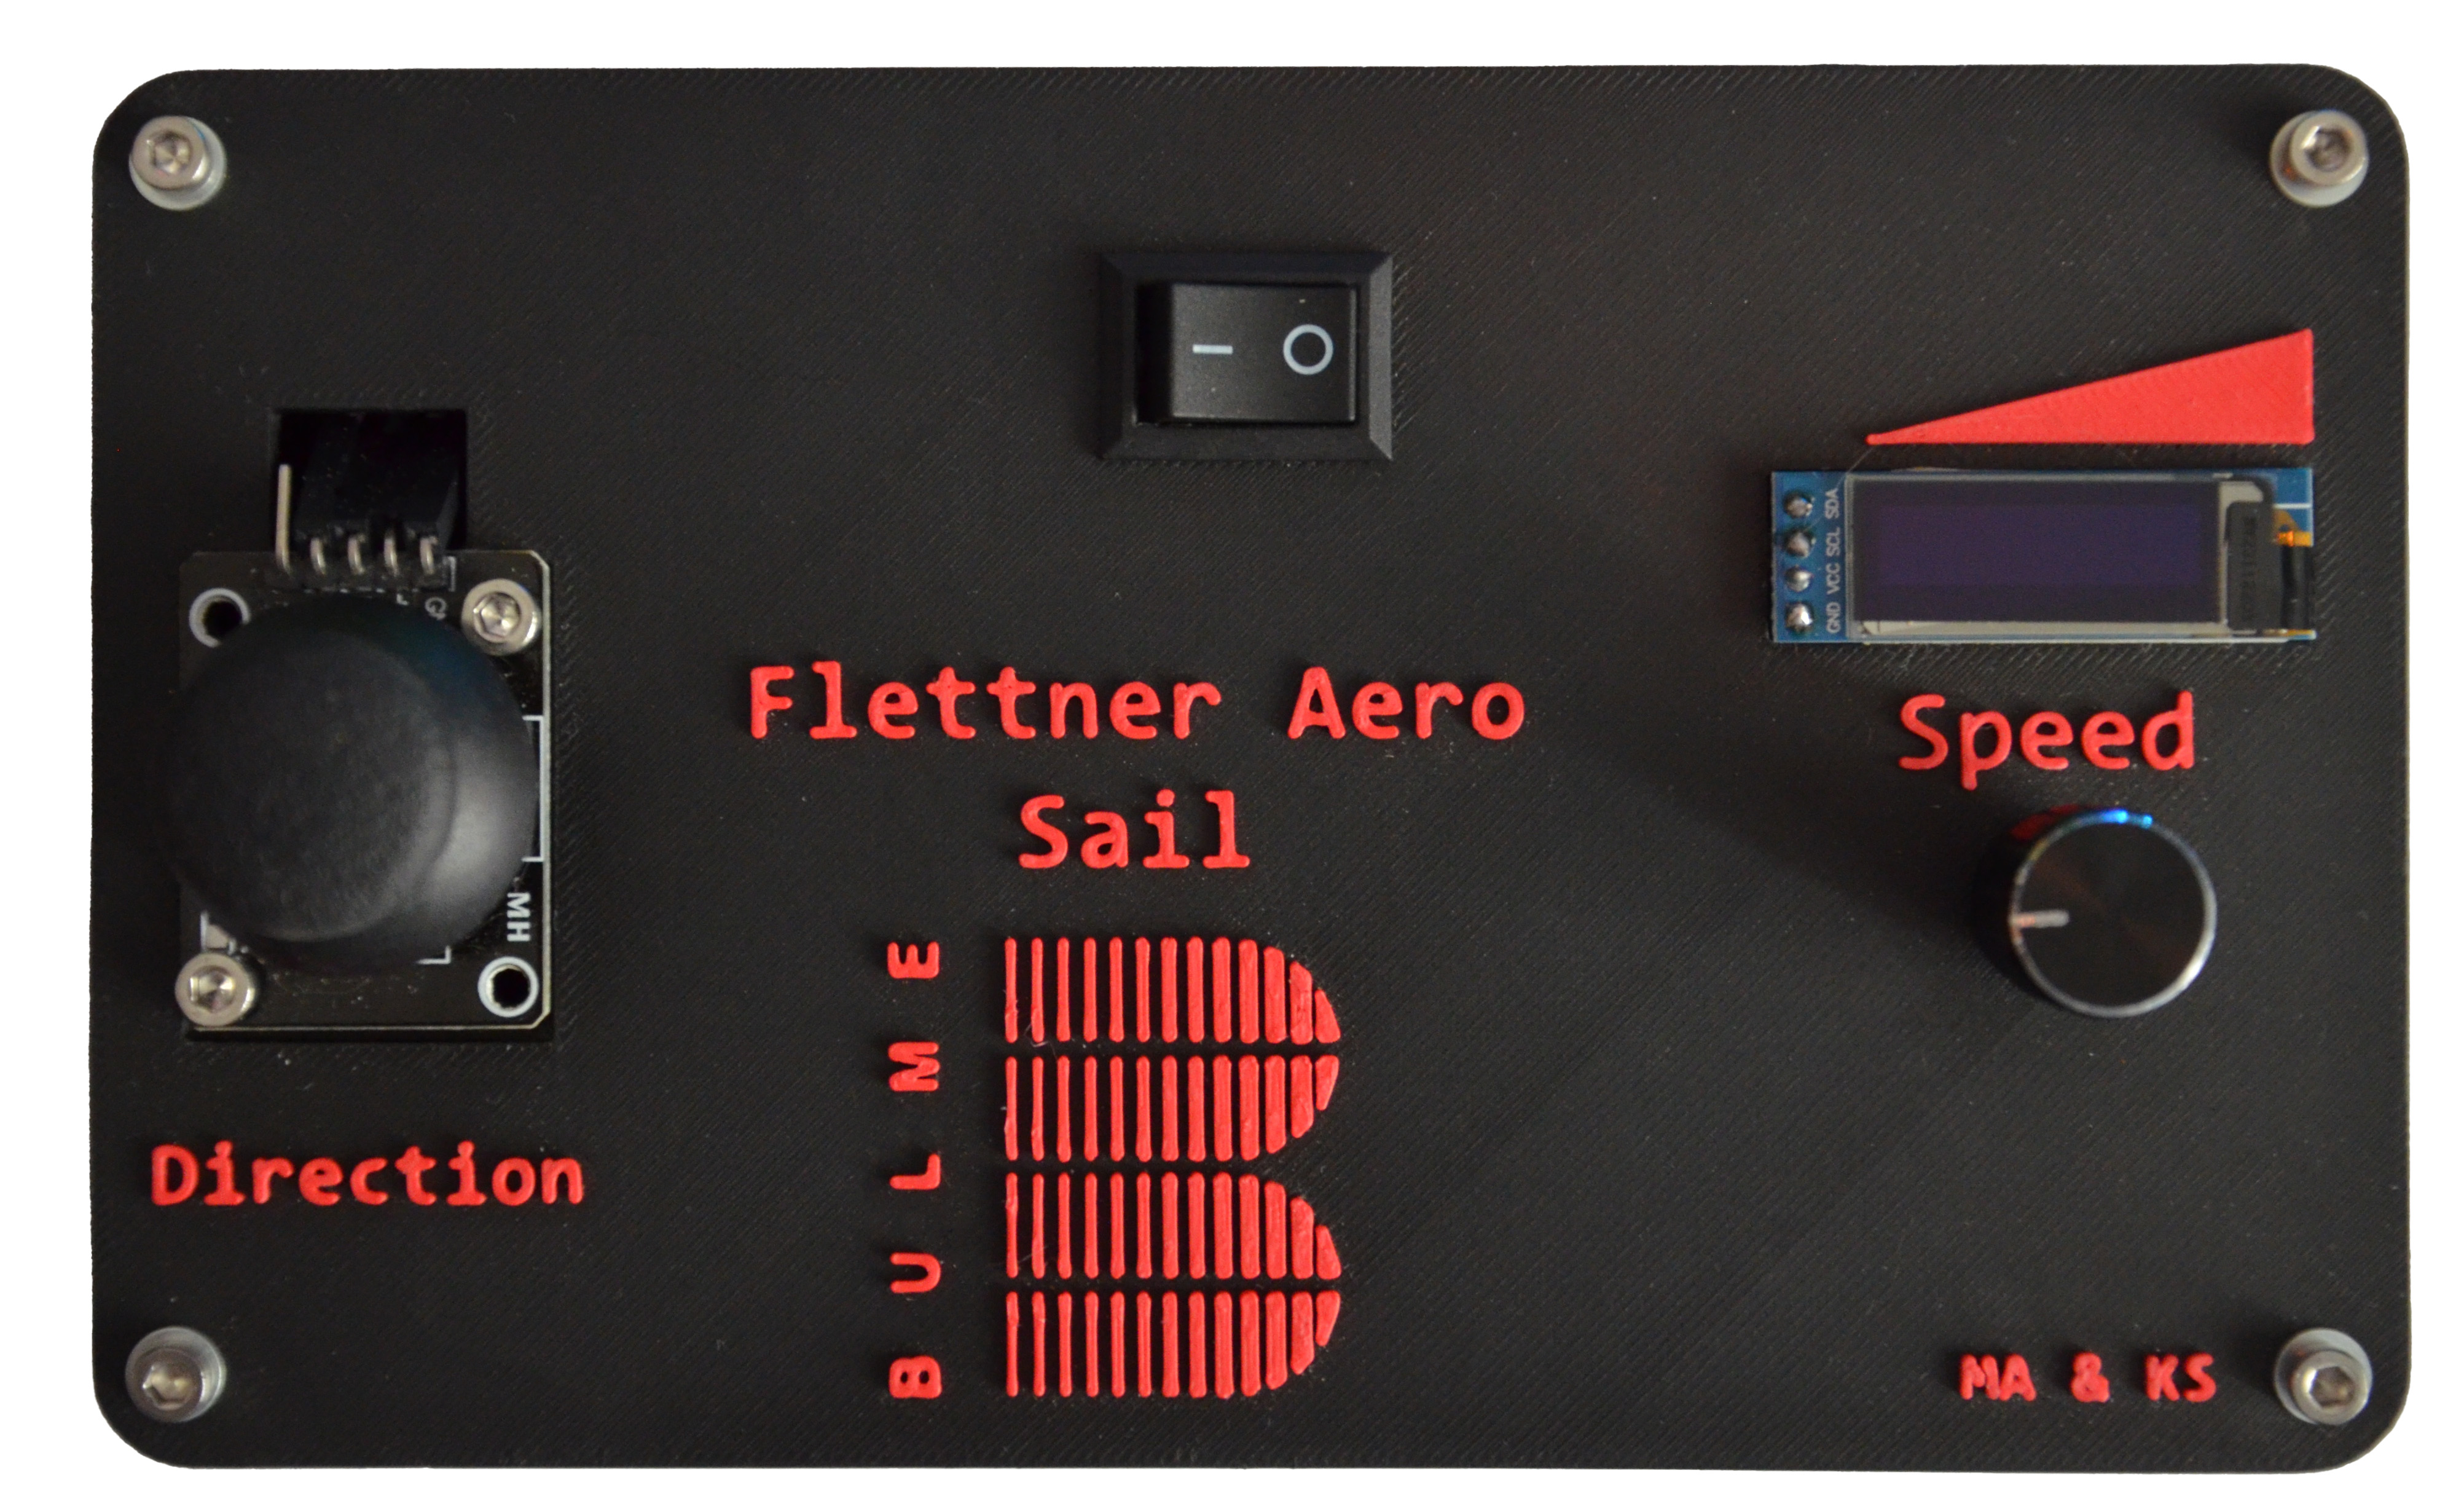
\includegraphics[width=\linewidth]{images/Controller ohne Hintergrund.jpg}
        \caption{Selbst entwickelter Controller}
        \label{fig:Controller}
    \end{minipage}
\end{figure}


Das Bedienkonzept des Controllers muss nur zwei Bewegungen ermöglichen. Erstens die einfache Regelung der Rotordrehzahl und zweitens die Auslenkung der Heckflosse. Nach dem Vergleich mehrerer Varianten fiel die Wahl auf die Kombination aus linkem Zwei-Achsen-Joystick und rechts angeordnetem Drehimpulsgeber für die Rotordrehzahl. Im Anfangsstadium des Projektes wurde mit dem Gedanken gespielt, den Aufbau eines Spielcontrollers zu übernehmen und die Geschwindigkeit des Rotors mit Hilfe eines Joysticks zu steuern. Dies erwies sich als unvernünftig, da man schwer eine konstante Geschwindigkeit halten und somit nicht akkurat messen konnte. Die Lösung dafür war, dass der linke Joystick bleibt und der rechte durch einen Drehimpulsgeber ausgetauscht wird. Somit konnte mit dem linken Joystick die Heckflosse einfach gesteuert und die Geschwindigkeit des Rotors einfach mit dem Drehimpulsgeber eingestellt werden. Zusätzlich zeigt ein kleines OLED-Display über einen \gls{i2c} einen Prozentwert der eingestellten Geschwindigkeit an.
\\[0.8em]
Wegen des knappen Zeitrahmens wurde das Design bewusst schlicht gehalten und es wurde sich mehr auf die Funktionalität der Steuerung fokussiert. Die Funktionalität ist hiermit komplett gegeben, obwohl die Ergonomie noch viele Anpassungen nötig hat. Als kleine Sicherheitseigenschaft wurde der Einsatz eines Schalters am Controller und auf dem Boot verwirklicht. Diese dienen bei unerwünschtem Verhalten für ein einfaches Abtrennen der Spannung.

\subsubsection*{Sender und Empfänger}

Die gesamte Steuerung basiert auf einem Sender- und Empfänger-Prinzip. Ein ESP32 dient als Steuerungseinheit für alle Eingaben wie Joystickbewegungen und Drehimpulse und überträgt die daraus resultierenden Steuerbefehle drahtlos an einen zweiten ESP32, der als Empfängereinheit fungiert und die entsprechenden Signale an die Aktoren weiterleitet.
% Bild von https://www.engineersgarage.com/what-is-esp-now/
\begin{figure}[H]
    \centering
    \includegraphics[width=0.85\linewidth]{images/ESP-Sender-Receiver.png}
    \caption{Sender und Empfänger Prinzip\cite{espnow_diagram}}
    \label{fig:sender-receiver}
\end{figure}
Das Boot an sich kann nur durch zwei Bewegungen gesteuert werden. Einmal durch das Andrehen des Motors, welcher dann den Flettner-Rotor \ref{fig:Rotor_Teil1} antreibt und einmal durch das Steuern der Heckflosse \ref{fig:Ruder} am Ende des Bootes. Für das Rotieren des Rotors eignet sich ein Drehimpulsgeber perfekt, da sich damit die Drehgeschwindigkeit präzise einstellen und konstant halten lässt. Die Rotorgeschwindigkeit lässt sich deshalb einfach durch den Drehimpulsgeber steuern. Durch das Drehen des Drehimpulsgebers im Uhrzeigersinn wird die Geschwindigkeit erhöht und das Drehen gegen den Uhrzeigersinn vermindert diese wieder. Darüber hinaus lässt sich durch Drücken des Drehimpulsgebers gleichzeitig der Rotor stoppen und die Drehrichtung des Rotors ändern.

\begin{figure}[H]
    \centering
    \begin{minipage}[b]{0.4\linewidth}
        \centering
        \includegraphics[width=\linewidth]{images/rotary-encoder.png}
        \caption{Drehimpulsgeber\cite{PiHut_RotaryEncoder}}
        \label{fig:rotary-encoder}
    \end{minipage}
    \hspace{1.2em}
    \begin{minipage}[b]{0.4\linewidth}
        \centering
        \includegraphics[width=\linewidth]{images/joystick.png}
        \caption{Joystick\cite{switch_dual_axis_joystick}}
        \label{fig:joystick}
    \end{minipage}
\end{figure}

Das Steuern der Heckflosse hingegen ist einfacher mit einem Joystick, da er eine besonders intuitive Handhabung ermöglicht. Den Joystick nach links zu drücken sorgt für Links-Bewegung der Flosse und den Joystick nach rechts zu drücken hat eine Rechts-Bewegung zu folge. In Abhängigkeit davon wie stark man den Joystick in eine Richtung lenkt, lenkt ebenso die Flosse unterschiedlich stark in eine Richtung. \newline
Da die Rotorgeschwindigkeit visuell nur schwer einzuschätzen ist, wird zusätzlich ein OLED-Anzeigemodul mit einer Auflösung von 128×32 Pixeln eingesetzt, das die aktuelle Geschwindigkeit in Prozent darstellt.


\subsubsection{Entprellen von Tastern}

Bei mechanischen Tastern schließt der Kontakt nicht sauber in einem einzigen Schritt: Beim Drücken oder Loslassen prallen die Kontaktflächen mehrmals kurz gegeneinander. Dadurch entstehen im Millisekunden-Bereich schnelle Pegelwechsel („Prellen“), die der Mikrocontroller als mehrere Tastendrücke auswerten könnte. Bei einem Drehimpulsgeber würden so falsche Messwerte entstehen, beim Joystick-Taster könnte eine einzige Betätigung gleich mehrere Betätigungen auslösen. Durch einen Entprell-Code, der einige Millisekunden den Taster ignoriert, wird sichergestellt, dass jede mechanische Aktion exakt einem digitalen Ereignis entspricht und die Steuerung zuverlässig arbeitet.

\paragraph*{Ausblick auf die Methodik}\leavevmode\\

Mit den vorangegangenen Abschnitten wurden alle \emph{Bausteine} der Fernsteuerung zusammengeführt – von der Auswahl des Funkprotokolls (ESP-NOW) über das Bedienkonzept aus Joystick und Dreh-Encoder bis zur sicheren Tasterabfrage mittels Entprell-Routine. Damit liegt nun ein vollständiges Hardware- und Softwaregerüst vor, das im nächsten Schritt praktisch erprobt werden kann.
\\[1em]
Kapitel \textbf{2 \emph{Methodik}} nimmt diesen Faden auf: Zunächst wird der \enquote{Proof of Concept} des Flettner-Prinzips an einem einfachen Versuchsaufbau beschrieben und ausgewertet. Anschließend folgt die schrittweise Konstruktion von Boot und Fernsteuerung sowie die detaillierte Verdrahtung beider Systeme. Den Abschluss bildet die Umsetzung der in Kapitel 1 skizzierten Steuerlogik in zwei ESP32-Firmwares, die eine bidirektionale, echtzeitfähige Kommunikation zwischen Controller und Boot ermöglichen.
\\[1em]
Der nun folgende Methodik-Teil zeigt also, \emph{wie} das zuvor ausgearbeitete Konzept in einen funktionsfähigen Prototyp übertragen, erprobt und iterativ verbessert wurde – und bildet damit die Brücke von der Theorie zur praktischen Validierung des Projekts.

%---------------------------------------------------------------------------------------------------
%---------------------------------------------------------------------------------------------------
% Kapitel 2
%---------------------------------------------------------------------------------------------------
%---------------------------------------------------------------------------------------------------
\newpage
\section{Methodik}

% Experimente, Durchführung partieller Codes und Erklärung

\subsection{\texorpdfstring{Erster Testaufbau um das physikalische Prinzip zu testen \textsubscript{[M]}}{Erster Testaufbau um das physikalische Prinzip zu testen [M]}}

Für den physikalischen Test wurde ein Versuchsaufbau unter Verwendung additiv gefertigter Komponenten realisiert. Ein 360°-Gelenk, ein Rotor sowie eine Motorhalterung wurden hierfür mittels CAD-Software (Fusion 360) konstruiert und anschließend im 3D-Druckverfahren hergestellt.. Die Abbildung \ref{fig:Konstruktionen erster Versuchsaufbau} zeigt die Konstruktionen. Zum Einsatz kam ein RC-DC-Motor Tamiya RS 540 SH.\cite{Datenblatt_Brushed_Motor} \newline
Der erste Versuch wurde mithilfe einer Holzstange realisiert, die mit dem Gelenk und dem Motor verbunden war. Dabei zeigte sich, dass die Holzstange bei höherer Drehzahl stark zu schwingen begann. Dieser Test wurde daraufhin abgebrochen, da es nicht möglich war, brauchbare Daten daraus zu gewinnen.

\begin{figure}[H]
    \centering
    \includegraphics[width=0.6\linewidth]{Konstruktion_erster_Versuchsaufbau.png}
    \caption{Konstruktionen für ersten Versuchsaufbau}
    \label{fig:Konstruktionen erster Versuchsaufbau}
\end{figure}

Daher wurde die Holzstange durch eine 10-mm-Gewindestange ersetzt und der Versuch erneut durchgeführt. Diese Konstruktion wies nur geringe Schwingungen auf, sodass der Test mit Einschränkungen durchgeführt werden konnte.
Die Konstruktion wurde an einer Latte befestigt, damit der Rotor frei hängt und in alle Richtungen über das 360°-Gelenk ausschwingen kann. Unterhalb wurde ein Koordinatensystem angebracht, um abzulesen, wie weit der Rotor in Abhängigkeit von Drehzahl und Windstärke ausgelenkt wird.
Zur Winderzeugung diente ein handelsüblicher Turmventilator, bei dem unterschiedliche Windstärken einstellbar sind. Der Motor wurde über ein Labornetzteil mit Energie versorgt. Den Versuchsaufbau kann man in Abbildung \ref{fig:1.Versuchsaufbau} sehen.\newline


\begin{figure}[H]
    \centering
    \includegraphics[width=0.9\linewidth]{images/1.Versuchsaufbau.jpg}
    \caption{Erster Versuchsaufbau}
    \label{fig:1.Versuchsaufbau}
\end{figure}

\subsection{\texorpdfstring{Problem beim Testaufbau \textsubscript{[K]}}{Problem beim Testaufbau [K]}}

Beim Test entstand durch die eingeschränkte Breite des Windstroms ein Pendeleffekt. 
\begin{figure}[H]
    \centering
    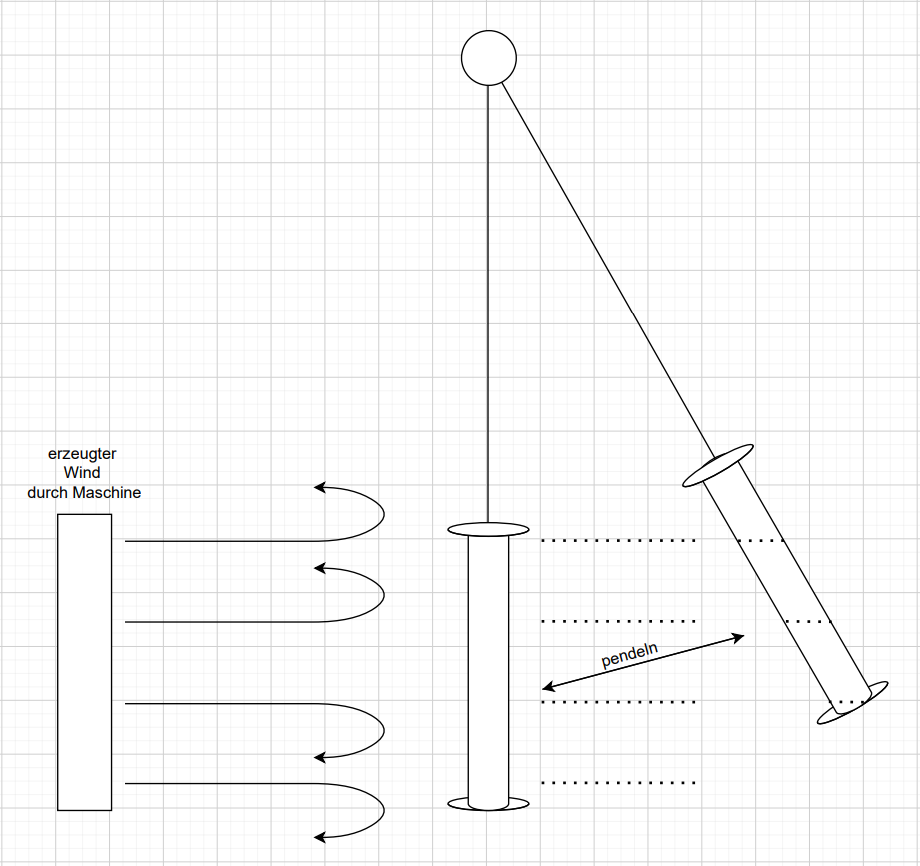
\includegraphics[width=0.9\linewidth]{images/Rotorpendeln.png}
    \caption{Skizze des aufgetretenen Pendeleffekts}
    \label{fig:SKizze Pendeleffekt}
\end{figure}
Wenn der Wind auf die rotierende Fläche traf, lenkte der Rotor wie gewünscht in eine Richtung aus. Dadurch trat jedoch das Problem auf, dass der Wind vom Ventilator nicht mehr direkt auf den Rotor traf, woraufhin dieser wieder zurückpendelte. Sobald der Wind dann erneut direkt auf den Rotor traf, erfolgte wieder eine Auslenkung. Dadurch entstand ein leichter Pendeleffekt, der das genaue Ablesen im Koordinatensystem erschwerte und inakkurat werden ließ. Für zukünftige Testversuche sollte daher ein System (genauer erläutert in Kapitel \ref{sec:Empfehlungsaufbau}) verwendet werden, welches den Windstrom kontinuierlich auf die Gesamtfläche des Rotors schießen kann.

\newpage

\subsection{\texorpdfstring{Auswertung des ersten Tests \textsubscript{[M]}}{Auswertung der ersten Tests [M]}}

Die Versuchsdaten wurden während des Tests manuell erfasst und anschließend in Microsoft Excel zu sehen in Abbildung \ref{fig:Auswertung 1 Excel} zur weiteren Auswertung übertragen. Ziel des Tests war es, den Einfluss verschiedener Parameter auf die Auslenkung des Rotors zu untersuchen.
Dabei wurden folgende Parameter systematisch variiert: die Ausgangsspannung des Netzteils, die Drehrichtung des Rotors sowie die Windgeschwindigkeit des Ventilators. \newline
\textbf{Spannung:} Die Tests wurden mit Spannungen im Bereich von 1 V bis 2 V durchgeführt. Spannungen außerhalb dieses Bereichs lieferten unter den gegebenen Testbedingungen keine verwertbaren Ergebnisse. \newline
\textbf{Windgeschwindigkeit:} Der eingesetzte Ventilator verfügte über drei Leistungsstufen. Stufe 1 erzeugte die geringste, Stufe 3 die höchste Luftgeschwindigkeit. \newline
\textbf{Drehrichtung des Rotors:} Durch Umpolen der Anschlussleitungen am Netzteil konnte die Drehrichtung des Rotors verändert werden, sodass eine Rotation im bzw. gegen den Uhrzeigersinn möglich war.

\begin{figure}[H]
    \centering
    \includegraphics[width=1\linewidth]{Auswertung1_groß.png}
    \caption{Auswertung 1 Excel}
    \label{fig:Auswertung 1 Excel}
\end{figure}


\textbf{Beobachtungen im Diagramm bei Rotor im Uhrzeigersinn:}\newline
Stufe 3 (x) ist konstant hoch (~6-6,5 cm) bis 1,3 V, sinkt dann leicht.\newline
Stufe 1 (x) zeigt klar abfallenden Trend.\newline
y-Auslenkung nimmt über alle Stufen leicht ab mit sinkender Spannung.\newline
Bei Stufe 3 ist die x-Auslenkung (bis ~6,5 cm) deutlich größer als bei Stufe 1 (~4 cm oder weniger), d.h. starker Wind + Rotation im Uhrzeigersinn = starke Wirkung. \newline
\textbf{Beobachtungen im Diagramm bei Rotor gegen den Uhrzeigersinn:}\newline
Kaum Veränderung der y-Werte - sie bleiben fast konstant bei 1 cm oder darunter.\newline
x-Werte fallen bei sinkender Spannung leicht ab, aber nicht so deutlich wie im Uhrzeigersinn-Test.
\newpage
Bei Stufe 1 sinken die Werte teilweise auf 0 cm y-Auslenkung, was auf eine praktisch nicht wirksame Rotorfunktion hinweist. \newline
\textbf{Fazit:}\newline
Effektiver Effekt entsteht vor allem bei Rotation im Uhrzeigersinn.\newline
Gegen den Uhrzeigersinn liefert kaum verwertbare Auslenkung - mögliche Erklärung: Strömungsrichtung des Ventilators + Drehrichtung kompensieren sich.\newline
Windstufe hat großen Einfluss - Stufe 3 erzeugt deutlich stärkere Auslenkung.\newline \newline
\textbf{Es wurde eine weitere Auswertung mit Excel durchgeführt. Dabei wurde der euklidische Abstand der x- und y-Koordinaten zum Ursprung (also der Betrag des Vektors) berechnet. Zusätzlich erfolgte eine Winkelberechnung in Grad, um die Richtung der Auslenkung relativ zur x-Achse zu bestimmen.}\newline \newline
Der Betrag des Vektors wurde mit dieser Formel berechnet:
\begin{equation}
r = \sqrt{x^2 + y^2}
\end{equation} \newline
Der Winkel wurde mit dieser Formel berechnet: 
\begin{equation}
\theta = \arctan\left(\frac{y}{x}\right)
\end{equation}

\begin{figure}[H]
    \centering
    \includegraphics[width=1\linewidth]{Auswertung2_groß.png}
    \caption{Auswertung 2 Excel}
    \label{fig:Auswertung 2 Excel}
\end{figure}

In Abbildung \ref{fig:Auswertung 2 Excel} ist erkennbar, wo die Auslenkung des Rotors am größten war. Diese Bereiche sind farblich in Grüntönen markiert, während die Bereiche mit der geringsten Auslenkung in Rottönen dargestellt sind. Die Farbcodierung basiert auf dem berechneten Betrag des Vektors, der den Abstand der x- und y-Koordinaten vom Ursprung beschreibt.
Es zeigt sich deutlich, dass mit zunehmender Windstufe (von Stufe 1 bis 3) auch die Auslenkungen größer werden. Gleichzeitig nimmt die Auslenkung mit abnehmender Spannung (unterhalb von ca. 1,3 V) spürbar ab, was auf eine reduzierte Effektivität des Rotors bei niedrigerer Antriebsspannung hinweist. 

\newpage

\subsection{\texorpdfstring{Konstruktion des Bootes und der Fernsteuerung\textsubscript{[M]}}{Konstruktion des Bootes und der Fernsteuerung [M]}}

Bei der Konstruktion des Bootes wurden verschiedene Katamaranbauweisen analysiert, um daraus Inspiration für das eigene Design zu gewinnen. Das Boot sollte nicht nur funktional überzeugen, sondern auch eine moderne Optik widerspiegeln. Darüber hinaus wurde darauf geachtet, eine ausgewogene Balance zwischen Stabilität und Effizienz zu erreichen. Die gesamte Konstruktion wurde mit Fusion 360 umgesetzt, wodurch sich die Bauteile präzise modellieren und optimal für den 3D-Druck exportieren ließen.\newline

Bis auf die Führungsstange inklusive Kugellager zur Rotorführung, einer Flanschverbindung, die Verbindungsrohre für die Mittelplatte und das Ruder zur Steuerung des Bootes wurden sämtliche Bauteile im 3D-Druckverfahren hergestellt. Da der 3D-Drucker in seinen Druckdimensionen begrenzt ist, wurden der Rotor, die Elektronikbox und die Schwimmer jeweils in zwei Teilen gefertigt. Der Rotor wurde so konstruiert, dass er eine Nut besitzt und die beiden Hälften passgenau ineinandergesteckt werden können. Die Schwimmer und die Elektronikbox hingegen wurden nach dem Druck mit einem speziellen, hochfesten 3D-Druck-Kleber dauerhaft verbunden. Zusätzlich wurde die Verbindungsstelle der Elektronikbox mit einer Dichtmasse versiegelt, um die Wasserdichtigkeit sicherzustellen. Die Schwimmer wurden aus dem hochfesten Filamenttyp PETG HF gefertigt, da dieses Material eine hohe Beständigkeit gegen Wasser, UV-Strahlung und erhöhte Temperaturen aufweist - Eigenschaften, die für den Einsatz im Außenbereich und im direkten Wasserkontakt besonders wichtig sind. Der Rotor hingegen wurde aus PLA Matte hergestellt, das sich durch eine matte, reflexionsarme Oberfläche und gute Druckbarkeit auszeichnet.\newline

Um die Wasserdichtigkeit der Schwimmer sicherzustellen, wurden diese zusätzlich mit einem speziellen Dichtspray Dichtol 2568 der Marke Diamant Polymer Solutions versiegelt. Sämtliche 3D-gedruckten Komponenten wurden anschließend sorgfältig zusammengesteckt und verschraubt, was eine stabile und modulare Gesamtstruktur ermöglichte.\cite{Technisches_Datenblatt_Dichtol}\newline

Bei der Elektronikbox wurde zusätzlich eine Nut mitkonstruiert, um ein Dichtband rund um diese einzukleben. Beim Verschrauben der Elektronikbox mit der Mittelplatte wird das Dichtband komprimiert und sorgt so für eine zuverlässige Abdichtung.

Beim Designprozess wurden kontinuierlich Anpassungen vorgenommen, wobei insbesondere die Überarbeitung des Rotors und des Rotorhalters hervorzuheben ist. Die erste Version des Rotors verfügte über keinen Führungsschaft mit Kugellagern, und auch der ursprüngliche Rotorhalter wurde ohne eine entsprechende Lagerführung konstruiert.

Bereits bei den ersten Versuchen, den Rotor mithilfe eines Motors in Rotation zu versetzen, zeigte sich deutlich, dass es zu unerwünschten Vibrationen kam. Daraufhin wurde entschieden, sowohl am Rotor als auch am Rotorhalter einen Schaft zu integrieren und diesen jeweils mit zwei Kugellagern auszustatten, um eine stabile und vibrationsarme Führung zu ermöglichen. Eine weitere Verbesserung des Rotorhalters wurde durch die Wahl einer anderen Filamentart erzielt. Zum Einsatz kam ASA CF, ein Material, das sich durch eine sehr hohe Steifigkeit auszeichnet. Dadurch konnten die Vibrationen zusätzlich reduziert werden.

Die Kugellager wurden mithilfe der Pausefunktion der 3D-Druck-Software Bambu Studio direkt in den Druckvorgang integriert. Dadurch konnten sie präzise und fest in die Bauteile eingebettet werden, was nicht nur den optimalen Sitz, sondern auch eine deutlich verbesserte Laufruhe und Stabilität der gesamten Konstruktion gewährleistet.


\subsubsection{Detailierte Angaben zu den Teilen die nicht 3D gedruckt wurden}

Als Führungsstange \ref{fig:Fuehrungsstange} für den Rotor wurde eine 350 mm lange Präzisionswelle aus Stahl mit einem Durchmesser von 8 mm gewählt. Sie zeichnet sich durch eine hohe Stabilität aus und eignet sich hervorragend für eine präzise lineare Führung des Rotors. Am oberen Ende des Rotors wurde die Welle mithilfe eines Flanschverbinders \ref{fig:Flanschverbinder} sicher befestigt.

Die Wahl einer stabilen Präzisionswelle aus Stahl ermöglicht eine zuverlässige Führung des Rotors über längere Betriebszeiten hinweg. Aufgrund der glatten Oberfläche und der Maßhaltigkeit eignet sich die Welle besonders gut für den Einsatz mit Kugellagern, wodurch eine ruhige und gleichmäßige Rotation gewährleistet wird. Dies trägt wesentlich zur Funktionssicherheit und zur mechanischen Stabilität der Gesamtkonstruktion bei.\newline


Bei der Wahl der Kugellager \ref{fig:Kugellager} fiel die Entscheidung auf das Modell 608 ZZ. Dieses Lager verfügt über einen Innendurchmesser von 8 mm, einen Außendurchmesser von 22 mm und eine Breite von 7 mm. Damit passt es ideal zur verwendeten Führungsstange und sorgt für eine spielfreie, präzise Führung.
Das Modell 608 ZZ ist beidseitig mit Metallabdeckungen (ZZ) versehen, wodurch es vor Staub und kleinen Partikeln geschützt ist - ein Vorteil, insbesondere im Einsatzumfeld mit rotierenden Bauteilen.\newline

Für die Verbindung der Mittelplatte wurde zunächst versucht die Verbindungsstangen im 3D- Druckverfahren herzustellen. Dies erwies sich jedoch als nicht stabil, da es beim wiederholten Auseinanderbauen zu Brüchen in den gedruckten Teilen kam. 

Als Lösung wurden zwei Aluminiumrohre mit einem Durchmesser von 10 mm einer Länge von 250 mm und einer Wandstärke von 1 mm verwendet. Diese stellten sich als deutlich stabiler heraus - nicht nur aufgrund der zuverlässigen Befestigungsmöglichkeiten für Schraubverbindungen, sondern auch, weil sie die gesamte Konstruktion erheblich gegen Verwindungen versteiften.

Zusätzlich bot die Wahl von Aluminium ein gutes Verhältnis zwischen Gewicht und Festigkeit, was zur Gesamtperformance des Bootes positiv beitrug.\newline


Für die Richtungssteuerung des Bootes wurde ein fertiges RC-Ruder \ref{fig:Ruder} aus einer hochwertigen Aluminiumlegierung verwendet. Dieses Material zeichnet sich durch seine hohe Stabilität, Korrosionsbeständigkeit und Rostfreiheit aus, was es ideal für den Einsatz in wasserbasierten Anwendungen macht. Das Ruder wurde ursprünglich für RC-Boote mit einer Länge von bis zu 85cm konzipiert und passte daher optimal zu den Anforderungen unseres Projekts.

Das Ruder verfügt über eine Ruderblatttiefe von 95 mm, eine Rahmenlänge von 60 mm, eine Rahmenbreite von 43 mm sowie einen Messingauslauf mit M4-Gewinde. Durch die präzise Fertigung und die stabile Bauweise konnte es einfach am Heck montiert werden. Die Entscheidung für dieses vormontierte Modell sparte Entwicklungszeit und bot gleichzeitig eine langlebige, funktionale Lösung für die Richtungslenkung. 

Zur aktiven Richtungslenkung wurde das Ruder mechanisch mit einem Servomotor verbunden, der die Position des Ruderblatts je nach Steuersignal exakt anpasst.

\newpage

\textbf{Bilder der verwendeten Teile}

% Link zum Bild der Führungsstange 
% https://www.amazon.de/dp/B0D2L59VPF?ref=ppx_yo2ov_dt_b_fed_asin_title&th=1

% Link zum Bild Flanschverbinder https://www.amazon.de/dp/B0833PM19X

\begin{figure}[H]
    \centering
    \begin{minipage}[b]{0.35\linewidth}
        \centering
        \includegraphics[width=\linewidth]{Bild Führungsstange.jpg}
        \caption{Führungsstange für Rotor\cite{Führungsstange_Rotor}}
        \label{fig:Fuehrungsstange}
    \end{minipage}
    \hspace{2.5em}  
    \begin{minipage}[b]{0.42\linewidth}
        \centering
        \includegraphics[width=\linewidth]{Flanschverbinder.jpg}
        \caption{Flanschverbinder\cite{Flanschverbinder}}
        \label{fig:Flanschverbinder}
    \end{minipage}
\end{figure}

% Link zum Kugellager https://www.amazon.de/dp/B08K936Y1Z

% Link zum Ruder https://www.amazon.de/dp/B0B4K33Q7X


\begin{figure}[H]
    \centering
    \begin{minipage}[b]{0.30\linewidth}
        \centering
        \includegraphics[width=\linewidth]{Kugellager 608ZZ.jpg}
        \caption{Kugellager 608ZZ\cite{Kugellager}}
        \label{fig:Kugellager}
    \end{minipage}
    \hspace{2.5em}  
    \begin{minipage}[b]{0.40\linewidth}
        \centering
        \includegraphics[width=\linewidth]{Ruder.jpg}
        \caption{Ruder\cite{Ruder}}
        \label{fig:Ruder}
    \end{minipage}
\end{figure}

\subsubsection{Konstruktion der Fernsteuerung}

Im Laufe der Diplomarbeit wurde die Entscheidung getroffen, die Fernsteuerung selbst zu konstruieren. Dies hatte den Vorteil, dass die gesamte verwendete Peripherie exakt dort platziert werden konnte, wo sie benötigt wird, und somit individuell an unsere Anforderungen angepasst werden konnte. Auch die Fernsteuerung wurde mithilfe von Fusion 360 entworfen und anschließend im 3D-Druckverfahren gefertigt. Gefertigt wurde das Gehäuse vollständig aus PLA Matte, wodurch eine hochwertige, matte Oberfläche erzielt wurde, die auch optisch zur Gesamtgestaltung des Projekts passt.


Ein weiterer Vorteil dieser Eigenkonstruktion war die Möglichkeit, die gesamte Elektronik - einschließlich des ESP32 - platzsparend und optimal im Gehäuse unterzubringen. Dadurch wurde eine saubere, kompakte Bauweise erreicht, die den Zugriff auf alle benötigten Komponenten deutlich erleichtert.

Zusätzlich konnte sowohl die Beschriftung als auch das äußere Design der Fernsteuerung frei gestaltet werden. Dadurch ließ sich nicht nur die Funktionalität, sondern auch die Benutzerfreundlichkeit gezielt verbessern.
\newpage


% Alle Konstruktionspläne des Bootes und des Controllers

\subsection{\texorpdfstring{Konstruktionspläne aller Bauteile\textsubscript{[M]}}{Konstruktionspläne aller Bauteile [M]}}

\textbf{Abbildung des gesamten Bootes\ref{fig:3D Ansichten Boot} in der 3D-Ansicht von Fusion 360}

\begin{figure}[H]
    \centering
    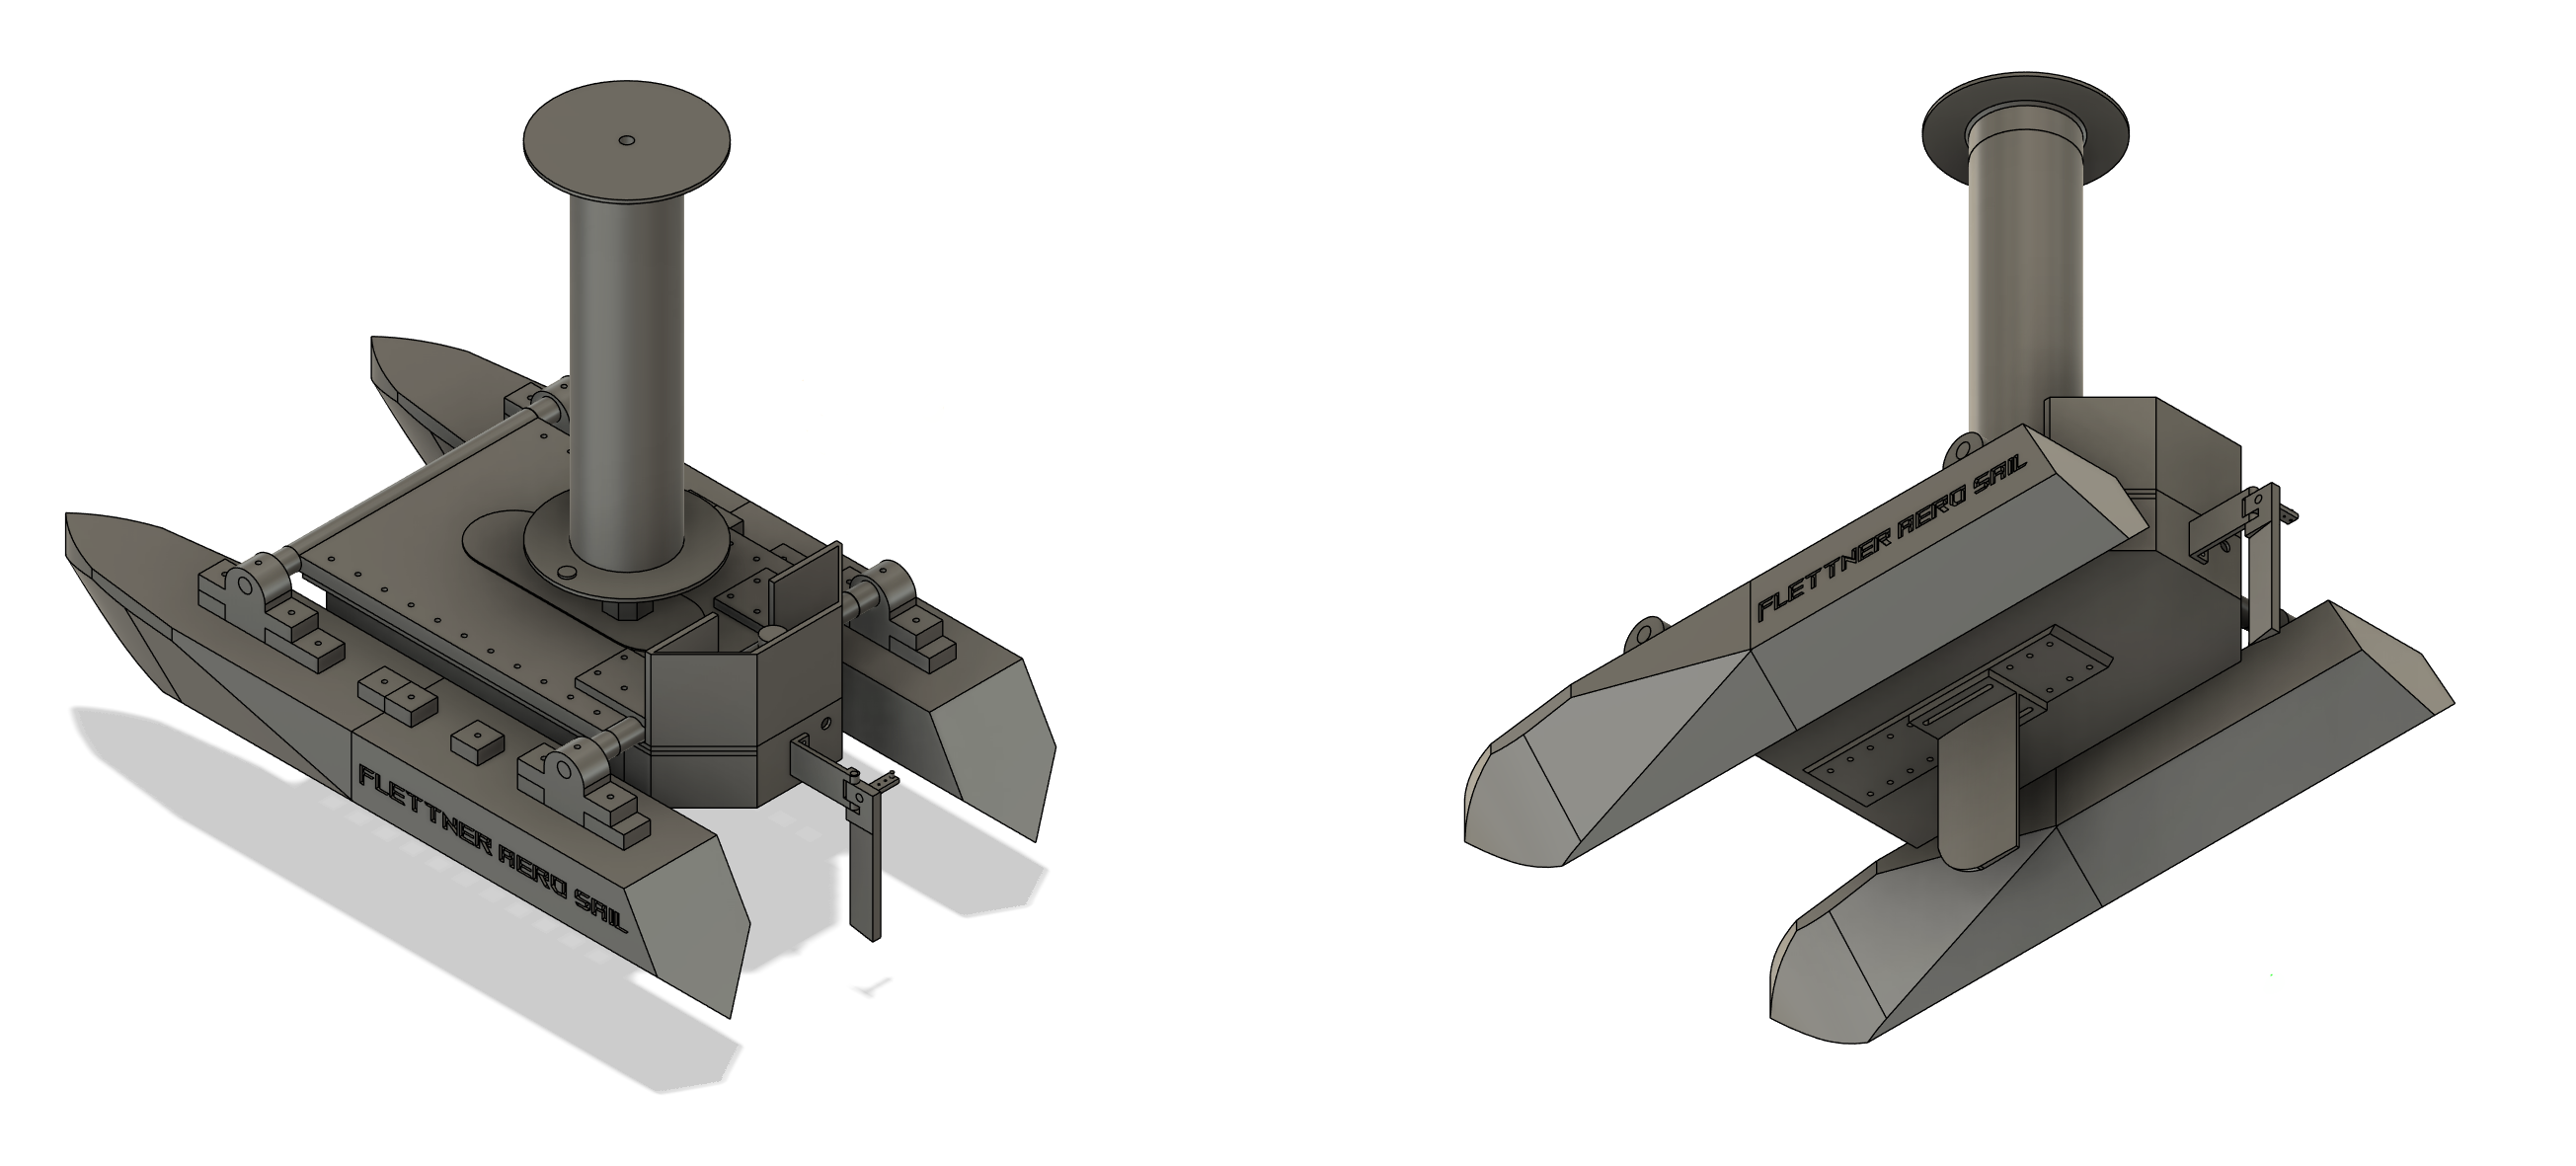
\includegraphics[width=1\linewidth]{3D Ansichten Boot.png}
    \caption{3D Ansichten Boot}
    \label{fig:3D Ansichten Boot}
\end{figure}


\textbf{Konstruktionsplan Schwimmer Teilstück vorne}

\begin{figure}[H]
    \centering
    \includegraphics[width=1.0\linewidth]{Schwimmer_Teilstück_vorne.pdf}
    \caption{Schwimmer Teilstück vorne}
    \label{fig:Schwimmer_vorne}
\end{figure}


\newpage

\textbf{Konstruktionsplan Schwimmer Teilstück hinten}

\begin{figure}[H]
    \centering
    \includegraphics[width=0.9\linewidth]{Schwimmer_Teilstück_hinten.pdf}
    \caption{Schwimmer Teilstück hinten}
    \label{fig:Schwimmer_hinten}
\end{figure}
 

\textbf{Konstruktionsplan Mittelplatte}

\begin{figure}[H]
    \centering
    \includegraphics[width=0.9\linewidth]{Mittelplatte.pdf}
    \caption{Mittelplatte}
    \label{fig:Mittelplatte}
\end{figure}

\textbf{Konstruktionsplan Rotor}

\begin{figure}[H]
    \centering
    \includegraphics[width=0.9\linewidth]{Rotor.pdf}
    \caption{Rotor Teil 1}
    \label{fig:Rotor_Teil1}
\end{figure}

\textbf{Konstruktionsplan Rotordeckel}

\begin{figure}[H]
    \centering
    \includegraphics[width=0.9\linewidth]{Rotordeckel.pdf}
    \caption{Rotordeckel}
    \label{fig:Rotordeckel}
\end{figure}


\textbf{Konstruktionsplan Rotorhalter}

\begin{figure}[H]
    \centering
    \includegraphics[width=0.9\linewidth]{Rotorhalter.pdf}
    \caption{Rotorhalter}
    \label{fig:Rotorhalter}
\end{figure}

\textbf{Konstruktionsplan Elektronikbox}

\begin{figure}[H]
    \centering
    \includegraphics[width=0.9\linewidth]{Elektronikbox.pdf}
    \caption{Elektronikbox}
    \label{fig:Elektronikbox}
\end{figure}

\textbf{Konstruktionsplan Verbindungsstange später Aluminium Rohr}

\begin{figure}[H]
    \centering
    \includegraphics[width=0.9\linewidth]{Verbindungsstange_250mm.pdf}
    \caption{Verbindungsstange}
    \label{fig:Verbindungsstange}
\end{figure}

\textbf{Konstruktionsplan Verbindungsstück}

\begin{figure}[H]
    \centering
    \includegraphics[width=0.9\linewidth]{Verbindungsstück.pdf}
    \caption{Verbindungsstück}
    \label{fig:Verbindungsstück}
\end{figure}


\textbf{Konstruktionsplan Zwischenstück}

\begin{figure}[H]
    \centering
    \includegraphics[width=0.9\linewidth]{Zwischenstück.pdf}
    \caption{Zwischenstück}
    \label{fig:Zwischenstück}
\end{figure}

\textbf{Konstruktionsplan Mittelfinne}

\begin{figure}[H]
    \centering
    \includegraphics[width=0.9\linewidth]{Mittelfinne.pdf}
    \caption{Mittelfinne}
    \label{fig:Mittelfinne}
\end{figure}

\textbf{Konstruktionsplan Dichtungsdeckel}

\begin{figure}[H]
    \centering
    \includegraphics[width=0.9\linewidth]{Dichtungsdeckel.pdf}
    \caption{Dichtungsdeckel}
    \label{fig:Dichtungsdeckel}
\end{figure}

\textbf{Konstruktionsplan Motorabdeckung}

\begin{figure}[H]
    \centering
    \includegraphics[width=0.9\linewidth]{Motorabdeckung.pdf}
    \caption{Motorabdeckung}
    \label{fig:Motorabdeckung}
\end{figure}

\textbf{Konstruktionsplan Controller unterer Teil}

\begin{figure}[H]
    \centering
    \includegraphics[width=0.9\linewidth]{Controller Teil 1.pdf}
    \caption{Controller Teil 1}
    \label{fig:Controller Teil 1}
\end{figure}

\textbf{Konstruktionsplan Controller oberer Teil}

\begin{figure}[H]
    \centering
    \includegraphics[width=0.9\linewidth]{Controller Teil 2.pdf}
    \caption{Controller Teil 2}
    \label{fig:Controller Teil 2}
\end{figure}


\subsection{\texorpdfstring{Schaltpläne zur Verkabelung von Boot und Controller \textsubscript{[M]}}{Schaltpläne zur Verkabelung von Boot und Controller [M]}}

\textbf{Schaltplan Boot}

\begin{figure}[H]
    \centering
    \includegraphics[width=0.8\linewidth]{Schaltplan Boot_1.png}
    \caption{Schaltplan Boot 1}
    \label{fig:Schaltplan Boot 1}
\end{figure}

\begin{figure}[H]
    \centering
    \includegraphics[width=0.75\linewidth]{Schaltplan Boot_2.png}
    \caption{Schaltplan Boot 2}
    \label{fig:Schaltplan Boot 2}
\end{figure}

\newpage
\textbf{Schaltplan Controller}

\begin{figure}[H]
    \centering
    \includegraphics[width=0.9\linewidth]{Schaltplan Controller_1.png}
    \caption{Schaltplan Controller 1}
    \label{fig:Schaltplan Controller 1}
\end{figure}

\begin{figure}[H]
    \centering
    \includegraphics[width=0.9\linewidth]{Schaltplan Controller_2.png}
    \caption{Schaltplan Controller 2}
    \label{fig:Schaltplan Controller 2}
\end{figure}

\subsubsection{\texorpdfstring{Stromversorgung für Boot und Fernsteuerung \textsubscript{[M]}}{Stromversorgung für Boot und Fernsteuerung [M]}}

Für die Stromversorgung des Bootes wird ein LiPo-Akku verwendet. Die Fernsteuerung wird über einen Batteriehalter mit vier AAA-Batterien betrieben.\cite{LiPo_Akku}\cite{Batterie_Halter}

\newpage

\subsection{\texorpdfstring{Umsetzung der Steuerung \textsubscript{[K]}}{Umsetzung der Steuerung [K]}}
\label{sec:Umsetzund der Steuerung}

Das Gesamtsystem besteht aus zwei ESP32-Boards, die über das drahtlose Protokoll ESP-NOW miteinander kommunizieren. Auf der Controller-Seite wird die Steuerungsschnittstelle samt Display und Eingabegeräten umgesetzt und auf der Boot-Seite erfolgt die Ansteuerung von Motor-ESC und Servo. Beide Firmwares sind in C++ realisiert und wurden mittels Visual Studio Code mit der Erweiterung PlatformIO programmiert. Im Folgenden wird der Aufbau und die Funktionsweise beider ESP32-Programme beschrieben, die gemeinsam die bidirektionale Steuerung und Regelung des Flettner-Rotorsystems ermöglichen. 


\subsubsection{Gemeinsame Datenstrukturen}
\label{sec:Gemeinsame Datenstrukturen}

Beide Programme verwenden dieselbe gepackte Datenstruktur, sodass jedes Byte an exakt derselben Position liegt. Diese Struktur enthält einen 32-Byte-langen Status-String, die rohen X- und Y-Werte des Joysticks, den Joystick-Taster, den umgerechneten PWM-Sollwert des Dreh-Encoders, dessen Taster und einen noch ungenutzten Platzhalter für eine Geschwindigkeitsbegrenzung. Die Geschwindigkeitsbegrenzung wird aktuell vom Boot-Programm verwaltet und sollte durch eine Erweiterung zukünftig vom Controller übernommen werden. Weil beide Seiten die Struktur identisch definieren, kann das gesamte Paket ohne weitere Konvertierung direkt kopiert werden.

\noindent\rule{\linewidth}{0.4pt}  % top stripe
\lstinputlisting[
]{codesnippets/controller/TransmitData.cpp}

\lstinputlisting[
  caption={Übertragene und empfangene Datenstruktur},
  label={lst:listing1-cpp}
]{codesnippets/boat/ReceivedData.cpp}
\noindent\rule{\linewidth}{0.4pt} % bottom stripe



\subsubsection{Funktionsweise der Controller-Firmware}
\label{sec:Funktionsweise der Controller-Firmware}

Zunächst initialisiert das Programm den seriellen Monitor, versetzt den ESP32 in den Station-Modus und startet anschließend die Programmteile für das OLED-Display, den Dreh-Encoder und ESP-NOW. 

\newpage
\noindent\rule{\linewidth}{0.4pt}  % top stripe
\lstinputlisting[
  caption={Controller Setup},
  label={lst:listing2-cpp}
]{codesnippets/controller/setup.cpp}
\noindent\rule{\linewidth}{0.4pt}\\[0.5em]  % bottom stripe
Während des gesamten Betriebs liest die Haupt-Schleife fortwährend die analogen Werte des Joysticks und die Zählwerte des Dreh-Encoders mit Hilfe der Aktualisierungsfunktionen aus. 

\begin{figure}[H]
    \centering
    \includegraphics[width=0.9\linewidth]{images/controllerFlowchart.png}
    \caption{Flowchart des Controllercodes}
    \label{Controlller-Flowchart}
\end{figure}

\newpage
\noindent\rule{\linewidth}{0.4pt}  % top stripe
\lstinputlisting[
  caption={Controller Loop},
  label={lst:listing3-cpp}
]{codesnippets/controller/loop.cpp}
\noindent\rule{\linewidth}{0.4pt}  % bottom stripe
Solange valueState.dataReady wahr ist, wird die Haupt-Schleife ausgeführt und aktualisiert somit alle Peripherie-Variablen. Sobald sich der Encoderwert ändert, rechnet das Programm den Zählerstand in einen Prozentwert zwischen null und hundert um, bestimmt daraus die gewünschte Drehzahl in Form eines PWM-Pulses zwischen 1000 und 2000 µs und aktualisiert die Anzeige. Jeder neue Sollzustand wird zusammen mit den aktuellen Joystick-Werten an das Boot gesendet. Drückt man den Encoder-Knopf, so invertiert das Programm einen booleschen Umschaltwert, setzt Geschwindigkeit und Zähler-Stand zurück und stellt dadurch die Drehrichtung um. Die Dreh-Impuls-Auswertung erfolgt per Interrupt, um auch bei schneller Betätigung keine Schritte zu verlieren. Ein Software-\gls{debouncing} unterdrückt Fehlauslösung, indem der Knopf erst als betätigt gilt, wenn nach seinem Zustandswechsel mindestens fünfzig Millisekunden vergangen sind.

\subsubsection{Joystickwerte abfangen}
\label{sec:Joystickwerte abfangen}

Die Joystickwerte werden fortlaufend in der Hauptschleife erfasst und direkt in die zu übertragende Datenstruktur geschrieben. Aufgrund des internen 12-Bit-\gls{adc}s des ESP32 liegen die Messwerte im Bereich von 0 bis 4095 und können deshalb fein quantisiert werden.
\newline\noindent\rule{\linewidth}{0.4pt}  % top stripe
\lstinputlisting[
  caption={Funktion für das Anzeigen am Controller-Display},
  label={lst:listing4-cpp}
]{codesnippets/controller/updateJoystickValues.cpp}
\noindent\rule{\linewidth}{0.4pt}  % bottom stripe



\subsubsection{Drehimpulsgebertaste auslesen}
\label{sec:Drehimpulsgebertaste auslesen}

Die Funktion handleEncoderButton() liest den Drucktaster des Dreh-Encoders aus, entprellt das Signal und führt bei jedem gültigen Tastendruck ein Stillstehen des Motors und eine Richtungsumkehr aus. Die Entprellzeit \texttt{DEBOUNCE\_DELAY\_MS} ist auf \SI{50}{\milli\second} festgelegt. Nach einer gültigen fallenden Flanke setzt die Funktion alle Geschwindigkeitswerte mit \texttt{resetValues()} zurück, sodass der Rotor sofort zum Stillstand kommt. Danach berechnet \texttt{determineSpeed()} den neuen PWM-Bereich. Da sowohl Entprellung als auch Richtungswechsel im Hauptprogramm ausgeführt werden, bleibt die Interrupt-Last gering und verursacht keine unerwünschten Unterbrechungen.

% Information von https://docs.arduino.cc/libraries/servo/

\noindent\rule{\linewidth}{0.4pt}  % top stripe
\lstinputlisting[
  caption={Funktion für das Auslesen der Drehimpulsgebertaste},
  label={lst:listing5-cpp}
]{codesnippets/controller/handleEncoderButton.cpp}
\noindent\rule{\linewidth}{0.4pt}  % bottom stripe


% https://wokwi.com/projects/344892392214626898
% wie man die Grafiken am Display erweitern kann
\subsubsection{Anzeige am OLED-Display}
\label{sec:Anzeige am OLED-Display}

Nach jeder Aktualisierung löscht das Programm den Bildschirm, schreibt die aktuelle Geschwindigkeit in Prozent in die erste Zeile und zeichnet darunter einen horizontalen Balken, dessen Länge dem Prozentwert entspricht. Auf diese Weise sieht der Benutzer in Echtzeit, wie stark der Rotor angesteuert wird. 
\newline\noindent\rule{\linewidth}{0.4pt}  % top stripe
\lstinputlisting[
  caption={Funktion für die Anzeige am Controller-Display},
  label={lst:listing6-cpp}
]{codesnippets/controller/updateDisplay.cpp}
\noindent\rule{\linewidth}{0.4pt}  % bottom stripe

\begin{figure}[htp]
\centering
\makebox[1em][l]{}%
\includegraphics[width=0.3\textwidth,valign=t]{images/Speed0.png}\hspace{1pt}%
\includegraphics[width=0.3\textwidth,valign=t]{images/Speed12.png}\hspace{1pt}%
\includegraphics[width=0.3\textwidth,valign=t]{images/Speed25.png}\\
\makebox[1em][l]{}%
\includegraphics[width=0.3\textwidth,valign=t]{images/Speed37.png}\hspace{1pt}%
\includegraphics[width=0.3\textwidth,valign=t]{images/Speed50.png}\hspace{1pt}%
\includegraphics[width=0.3\textwidth,valign=t]{images/Speed62.png}\\
\makebox[1em][l]{}%
\includegraphics[width=0.3\textwidth,valign=t]{images/Speed75.png}\hspace{1pt}%
\includegraphics[width=0.3\textwidth,valign=t]{images/Speed87.png}\hspace{1pt}%
\includegraphics[width=0.3\textwidth,valign=t]{images/Speed100.png}
\caption{Prozentuelle Anzeige der Geschwindigkeit am Controller\label{fig:SpeedDisplay}}
\end{figure}

Die Prozentangabe stellt nicht den theoretisch erreichbaren Maximalwert dar, sondern bereits den durch den Faktor \texttt{SPEED\_IN\_PERCENT} abgesenkten Wert. Diese Variable begrenzt die Ober- und Untergrenze der PWM-Impulse und skaliert damit die effektive Drehzahl. Die Anzeige spiegelt somit den \emph{skalierten} Wert von 0 bis 100\% wider.

\subsubsection{Datenübertragung mit ESP-NOW}
\label{sec:Datenübertragung mit ESP-NOW}

Nach der Initialisierung registriert das Programm die MAC-Adresse der Boot-Platine als Peer und kann die Befehle damit gezielt an das Gerät mit der entsprechenden Adresse weiterleiten. Jedes Mal, wenn ein Datenpaket verschickt wurde, ruft die ESP-NOW-Bibliothek den Callback onSent() auf.
\newline\noindent\rule{\linewidth}{0.4pt}  % top stripe
\lstinputlisting[
  caption={Funktion, welche das ESP-NOW Protokoll aufsetzt},
  label={lst:listing7-cpp}
]{codesnippets/controller/initializeESPNOW.cpp}
\noindent\rule{\linewidth}{0.4pt}  % bottom stripe
\newpage
\noindent\rule{\linewidth}{0.4pt}  % top stripe
\lstinputlisting[
  caption={ESP-NOW Callback Funktion},
  label={lst:listing8-cpp}
]{codesnippets/controller/onSent.cpp}
\noindent\rule{\linewidth}{0.4pt}\\[0.5em]  % bottom stripe
Da die Verbindung von der Boot-Seite zeitlich kontrolliert wird und sich somit um die Sicherheit kümmert, muss von der Controller-Seite nichts weiteres getan werden.

\subsubsection{Funktionsweise der Boot-Firmware}
\label{sec:Funktionsweise der Boot-Firmware}

Die Boot-Firmware startet ebenfalls in den STA-Modus, bindet das Servo und den ESC an die vorgesehenen Pins und wartet anschließend auf hereinkommende Daten.
\newline\noindent\rule{\linewidth}{0.4pt}  % top stripe
\lstinputlisting[
  caption={Boot Setup},
  label={lst:listing9-cpp}
]{codesnippets/boat/setup.cpp}
\noindent\rule{\linewidth}{0.4pt}\\[0.5em]  % bottom stripe
Trifft ein gültiges Datenpaket ein, kopiert das Empfangs-Callback die Nutzdaten in die lokale Struktur, speichert den aktuellen Zeitpunkt in lastUpdate und setzt eine Flagge, die signalisiert, dass neue Daten vorliegen. 
\newline\noindent\rule{\linewidth}{0.4pt}  % top stripe
\lstinputlisting[
  caption={Boot Setup},
  label={lst:listing10-cpp}
]{codesnippets/boat/onReceive.cpp}
\noindent\rule{\linewidth}{0.4pt}\\[0.5em]  % bottom stripe
Im Haupt-Loop prüft das Programm zuerst, ob seit der letzten Aktualisierung mehr als eine Sekunde vergangen ist. Ist dies der Fall, nimmt es an, dass die Funkverbindung unterbrochen wurde, stellt das Servo auf die Mittelstellung und sendet einen Neutral-Puls von 1500 µs plus kleinem Offset an den ESC, damit der Rotor sicher stoppt.
\newline\noindent\rule{\linewidth}{0.4pt}  % top stripe
\lstinputlisting[
  caption={Boat Hauptschleife},
  label={lst:listing11-cpp}
]{codesnippets/boat/loop.cpp}
\noindent\rule{\linewidth}{0.4pt}  % bottom stripe
\begin{figure}[H]
    \centering
    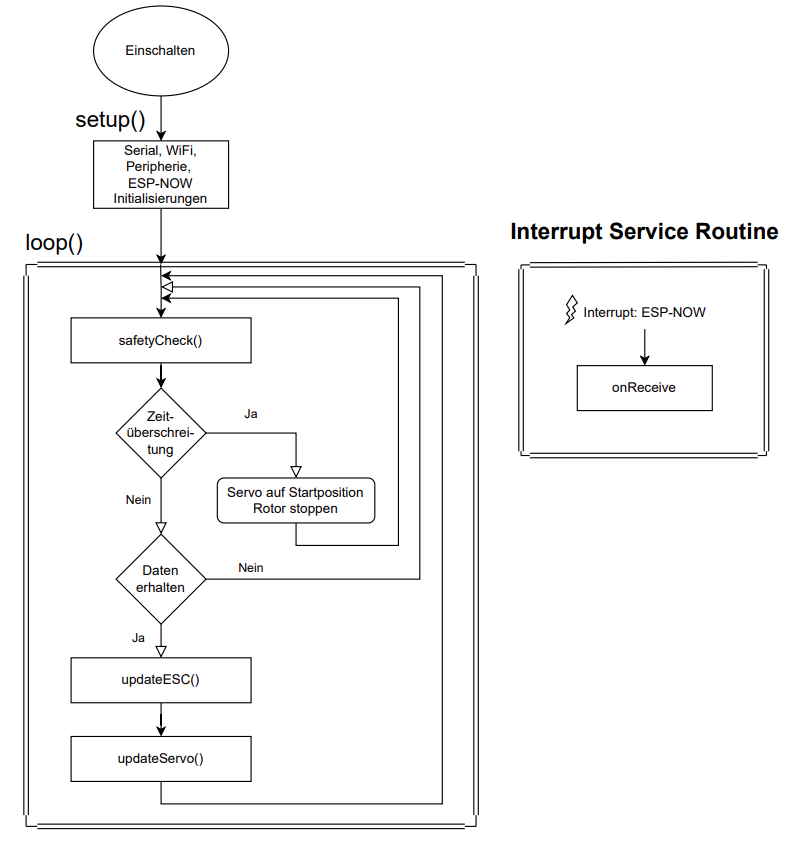
\includegraphics[width=0.9\linewidth]{images/boatFlowchart.png}
    \caption{Flowchart des Bootcodes}
    \label{Boat-Flowchart}
\end{figure}

\subsubsection{Ansteuerung von ESC und Servo}
\label{sec:Ansteuerung von ESC und Servo}

Das ESC-Update vergleicht den PWM-Wert aus dem Datenpaket mit der Neutralmarke von 1500 µs. Liegt er darüber, so begrenzt die Routine den Wert auf maximal 2000 µs minus Neutral-Offset, weil der Regler sonst sofort in Vollgas überginge. Liegt er darunter, so ist der minimale Puls 1000 µs. Nach der Begrenzung addiert das Programm einen Offset von zwanzig Mikrosekunden, weil der verwendete Regler erfahrungsgemäß erst leicht oberhalb der geometrischen Mitte wirklich stoppt.
\newline\noindent\rule{\linewidth}{0.4pt}  % top stripe
\lstinputlisting[
  caption={Funktion für das Aktualisieren der ESC-Werte},
  label={lst:listing12-cpp}
]{codesnippets/boat/updateESC.cpp}
\noindent\rule{\linewidth}{0.4pt}\\[0.5em]  % bottom stripe
Die Servoroutine verwendet ausschließlich den Y-Wert des Joysticks. Wenn dieser Wert die definierte Totzone überschreitet, rechnet das Programm ihn in einen Winkel zwischen 25 und 155 Grad um. Dadurch folgt die Flosse sauber der Lenkung, ohne dass sie bei minimalen Joystickbewegungen unerwünscht zu zittern beginnt.
\newline\noindent\rule{\linewidth}{0.4pt}  % top stripe
\lstinputlisting[
  caption={Funktion für das Aktualisieren der Servo-Werte},
  label={lst:listing13-cpp}
]{codesnippets/boat/updateServo.cpp}
\noindent\rule{\linewidth}{0.4pt}  % bottom stripe


\subsubsection*{Sicherheits- und Überwachungsmechanismen}
\label{sec:Sicherheits- und Überwachungsmechanismen}

Sollte aus unerwarteten Gründen die Verbindung zwischen Controller und Boot verloren gehen, dann wird über eine Sicherheitsüberprüfung das Boot zum Stillstand gebracht. Der gesamte Sicherheitsmechanismus ist im Boot verankert, weil dort unmittelbar die gefährlichen Aktoren angeschlossen sind. Die Firmware vergleicht kontinuierlich die aktuelle Zeit mit dem Zeitstempel des letzten gültigen Pakets. 
\newline\noindent\rule{\linewidth}{0.4pt}  % top stripe
\lstinputlisting[
  caption={Sicherheitsfunktion für den Stillstand},
  label={lst:listing14-cpp}
]{codesnippets/boat/safetyCheck.cpp}
\noindent\rule{\linewidth}{0.4pt}\\[0.5em]  % bottom stripe
Wenn das Zeitintervall das definierte Limit von einer Sekunde überschreitet, schaltet sie alle Aktoren in einen sicheren Ruhezustand. Gleichzeitig wird die Flagge dataReceived auf \enquote{false} gesetzt, sodass keine alten Werte mehr ausgewertet werden. Diese Maßnahme verhindert, dass ein Rotor weiterläuft oder der Servo in einer extremen Stellung verharrt, falls der Funkkontakt abreißt oder der Controller ausfällt.

% https://lastminuteengineers.com/handling-esp32-gpio-interrupts-tutorial/
\subsubsection{Interrupt-Verarbeitung im Controller}
\label{sec:Interrupt-Verarbeitung im Controller}

Die beiden Interrupt-Routinen updateEncoderA() und updateEncoderB() lesen jeweils die Pegel der A- und B-Leitung des Dreh-Encoders und entscheiden anhand ihrer Kombination, ob der Zähler dekrementiert oder inkrementiert werden muss. 
\newline\noindent\rule{\linewidth}{0.4pt}  % top stripe
\lstinputlisting[
  caption={Drehencoder \gls{isr} Funktionen},
  label={lst:listing15-cpp}
]{codesnippets/controller/updateEncoder.cpp}
\noindent\rule{\linewidth}{0.4pt}\\[0.5em]  % bottom stripe
Anschließend begrenzt eine constrain()-Anweisung den Zählerstand auf den Bereich null bis hundert, damit falsche Werte durch mechanisches Prellen oder sehr schnelles Drehen ausgeschlossen sind. IRAM\_ATTR\cite{espidf_memory_iram} sorgt dafür, dass der Compiler die Routinen in das schnellere Instruktions-RAM legt und somit kurze Latenzen garantiert.

\subsubsection{Berechnung des PWM-Sollwerts}
\label{sec:Berechnung des PWM-Sollwerts}
In der Funktion determineSpeed() nimmt das Programm den aktuellen prozentualen Geschwindigkeitswert und bildet daraus einen Bereich zwischen 1500 µs und jeweils 500 µs ober- oder unterhalb der Mitte. 1500 µs entsprechen der Neutralstellung, 1000 µs dem maximalen Linksdreh und 2000 µs dem maximalen Rechtsdreh des Motors.
\newline\noindent\rule{\linewidth}{0.4pt}  % top stripe
\lstinputlisting[
  caption={Drehencoder ISR Funktionen},
  label={lst:listing16-cpp}
]{codesnippets/controller/determineSpeed.cpp}
\noindent\rule{\linewidth}{0.4pt}\\[0.5em]  % bottom stripe

Dieser Maximalhub wird zusätzlich mit einem variablen Faktor SPEED\_IN\_PERCENT multipliziert, sodass sich die Ober- und Untergrenzen der Drehzahl mit nur einer Konstanten global reduzieren lassen. Wenn der Reverse-Modus aktiv ist, findet die Abbildung auf der gegenüberliegenden Seite der Neutralposition statt, sodass positive Prozentwerte zu höheren Pulsbreiten führen, die oberhalb von 1500 µs liegen. \newline

Bei der ternären Abfrage sieht die Berechnung wie folgt aus:
\begin{equation}
    1500 \pm (500*(\texttt{SPEED\_IN\_PERCENT}/100))
\end{equation}

Sie reicht somit von 1500 nach 1000 und von 1500 nach 2000 in Abhängigkeit von der booleschen Variable \texttt{valueState.reverseState} und der prozentualen Geschwindigkeitsvariable \texttt{SPEED\_IN\_PERCENT}.


\subsubsection{Anzeige- und Bedienkomfort}
\label{sec:Anzeige- und Bedienkomfort}

Da sämtliche Updates erst in den RAM-Puffer gegeben und erst danach gesammelt an das Display geschickt werden, treten keinerlei sichtbare Flackereffekte auf. Die Deckkraft des gefüllten Balkens gibt dem Benutzer ein unmittelbares Feedback über die eingestellte Leistung, während der numerische Prozentwert eine präzise Kontrolle erleichtert. Drückt der Nutzer den Dreh-Encoder-Knopf, wird der Bildschirm sofort gelöscht, Geschwindigkeit und Richtung werden zurückgesetzt, und der Nutzer erhält visuell die Bestätigung, dass eine neue Fahrtrichtung gewählt wurde.

\subsubsection{Konfigurations-Konstanten}
\label{sec:Konfigurations-Konstanten}

Früher definierte man feste Zahlen oder Zeichenketten in C++ oft per \verb|#define|. Dabei ersetzt der Präprozessor den Namen noch vor der eigentlichen Übersetzung wortwörtlich durch den Wert. Das ist zwar bequem, hat aber seine Nachteile: Der ersetzte Text besitzt keinen Typ, kann sich unbemerkt durch das ganze Projekt schleichen und ist im Debugger nicht sichtbar. Mit \verb|static constexpr| erreicht man dasselbe. Der Wert steht bereits zur Kompilierzeit fest, ist nur deutlich ordentlicher. Die Konstante hat einen klaren Typ, respektiert Namensräume und lässt sich debuggen. Seit C++17 sind solche Konstanten außerdem \emph{inline} und dürfen gefahrlos in Headern stehen, ohne doppelte Definitionen zu verursachen. Daher greift man heute für feste Werte fast immer zu \verb|static constexpr| statt \verb|#define|.
\\[1em]
Im Folgenden werden die benutzten Konstanten näher erläutert:
\begin{table}[H]
\centering
\renewcommand{\arraystretch}{1.5}
\begin{tabular}{|p{5cm}|p{10cm}|}
\hline
\rowcolor{gray!30}
\textbf{Konstante} & \textbf{Kurzbeschreibung \&  Anpassungsmöglichkeiten} \\
\hline
CONTROLLER\_MAC &
\begin{tabular}[t]{@{}l@{}}
MAC-Adresse des Hand-Controllers für die drahtlose 
\\[-0.4em]ESP-NOW-Verbindung. Muss über einen eigenen Code 
\\[-0.4em]ausgelesen werden.
\end{tabular} \\
\hline
BOAT\_MAC & 
\begin{tabular}[t]{@{}l@{}}
MAC-Adresse des Boots für die Drahtlose ESP-NOW-
\\[-0.4em]Verbindung. Muss ebenfalls über einen eigenen Code 
\\[-0.4em]ausgelesen werden.
\end{tabular} \\
\hline
JOYSTICK\_X\_PIN & 
\begin{tabular}[t]{@{}l@{}}
ADC-Eingang am ESP32, der über analogRead() die 
\\[-0.4em]Werte für die X-Achse des Joysticks ausliest. Wird 
\\[-0.4em]standardmäßig mit einer 12-Bit Auflösung gelesen. 
\\[-0.4em]Kann auch mit weniger als 12-Bit Auflösung verwendet 
\\[-0.4em]werden.
\end{tabular} \\
\hline
JOYSTICK\_Y\_PIN & 
\begin{tabular}[t]{@{}l@{}}
ADC-Eingang am ESP32, der über analogRead() die 
\\[-0.4em]Werte für die Y-Achse des Joysticks ausliest. Wird 
\\[-0.4em]standardmäßig mit einer 12-Bit Auflösung gelesen. 
\\[-0.4em]Kann auch mit weniger als 12-Bit Auflösung verwendet 
\\[-0.4em]werden.
\end{tabular} \\
\hline
ENCODER\_CLK & 
\begin{tabular}[t]{@{}l@{}}
GPIO-Leitung \enquote{A/CLK} des Drehencoders.
\end{tabular} \\
\hline
ENCODER\_DT & 
\begin{tabular}[t]{@{}l@{}}
GPIO-Leitung \enquote{B/DT} des Drehencoders.
\end{tabular} \\
\hline
ENCODER\_BTN & 
\begin{tabular}[t]{@{}l@{}}
GPIO-Eingang für den Drucktaster im Drehencoder.
\end{tabular} \\
\hline
SDA\_PIN & 
\begin{tabular}[t]{@{}l@{}}
I2C-SDA-Leitung für das OLED-Display. Muss theore-
\\[-0.4em]tisch nicht definiert werden, da SDA bei dem 30 und 
\\[-0.4em]32-Pin Modell immer auf GPIO21 liegt; dient mehr als 
\\[-0.4em]Übersicht.
\end{tabular} \\
\hline
SCL\_PIN & 
\begin{tabular}[t]{@{}l@{}}
I2C-SCL-Leitung für das OLED-Display. Muss theore-
\\[-0.4em]tisch nicht definiert werden, da SCL bei dem 30 und 
\\[-0.4em]32-Pin Modell immer auf GPIO22 liegt; dient mehr als 
\\[-0.4em]Übersicht.
\end{tabular} \\
\hline
TESTING\_ACTIVE & 
\begin{tabular}[t]{@{}l@{}}
Erlaubt durch serielle Ausgabe das Abfangen der Informationen.
\end{tabular} \\
\hline
DEBOUNCE\_DELAY\_MS & 
\begin{tabular}[t]{@{}l@{}}
Entprellzeit in Millisekunden für Taster- und Encoder-
\\[-0.4em]Ereignisse. 
\end{tabular} \\
\hline
\end{tabular}
\label{tab:controllerconstants1}
\end{table}

\begin{table}[H]
\centering
\renewcommand{\arraystretch}{1.5}
\begin{tabular}{|p{5cm}|p{10cm}|}
\hline
\rowcolor{gray!30}
\textbf{Konstante} & \textbf{Kurzbeschreibung \&  Anpassungsmöglichkeiten} \\
\hline
SPEED\_IN\_PERCENT & 
\begin{tabular}[t]{@{}l@{}}
Geschwindigkeitswert in Prozent. 100\% lassen den Mo-
\\[-0.4em]tor auf das Maximum fahren. Dient in dem Programm 
\\[-0.4em]zur Limitierung des Motors. 
\end{tabular} \\
\hline
SCREEN\_WIDTH & 
\begin{tabular}[t]{@{}l@{}}
Pixelbreite des verwendeten OLED-Displays.(128 Pixel)
\end{tabular} \\
\hline
SCREEN\_HEIGHT & 
\begin{tabular}[t]{@{}l@{}}
Pixelhöhe des verwendeten OLED-Displays.(32 Pixel)
\end{tabular} \\
\hline
OLED\_ADDRESS & 
\begin{tabular}[t]{@{}l@{}}
I2C-Adresse des Displays. (0x3C)
\end{tabular} \\
\hline

\end{tabular}
\caption{Verwendete Konstanten im Controller}
\label{tab:controllerconstants2}
\end{table}



\noindent\rule{\linewidth}{0.4pt}  % top stripe
\lstinputlisting[
  caption={Drehencoder ISR Funktionen},
  label={lst:listing17-cpp}
]{codesnippets/controller/configurationConstants.cpp}
\noindent\rule{\linewidth}{0.4pt}  % bottom stripe
\\[-0.8em]

\subsubsection*{Änderungen der Konstanten}
\label{sec:Änderung der Konstanten}

Die Konstanten sind jeweils an den konkreten Einsatzzweck anzupassen. Kommen neue ESP-Boards zum Einsatz, sollte man zunächst die MAC-Adresse jedes Moduls mit einem kleinen Hilfsprogramm auslesen und anschließend im Quellcode hinterlegen; erst dann kann die Funkverbindung aufgebaut werden. Alternativ lässt sich die MAC-Adresse auch direkt per Programmcode überschreiben(jedoch nur solange das Board nicht zurückgesetzt wird, weil es die wahre MAC-Adresse, die vom Hersteller vorgegeben ist, nicht überschreiben kann), ohne sie vorher auszulesen – die Zieladresse muss dann allerdings fix im Code stehen. Die folgenden Code-Snippets von Random Nerd Tutorials\cite{rnt_mac} zeigen beide Varianten:

\newpage
\noindent\rule{\linewidth}{0.4pt}  % top stripe
\lstinputlisting[
  caption={MAC-Adresse lesen},
  label={lst:listing18-cpp}
]{codesnippets/Get_MAC_Address.cpp}
\noindent\rule{\linewidth}{0.4pt}  % bottom stripe
\\[-0.8em]

Der gezeigte Quellcode liest nach dem Hochfahren des Wi-Fi-Stacks die werksseitige MAC-Adresse des ESP32 aus und gibt sie als formatierten Hex-String auf der seriellen Konsole aus. So lässt sich die eindeutige Kennung eines neuen Boards rasch ermitteln und später im Gegenstück hinterlegen, ohne noch weitere Schritte im Sketch ausführen zu müssen.

\noindent\rule{\linewidth}{0.4pt}  % top stripe
\lstinputlisting[
  caption={MAC-Adresse festlegen},
  label={lst:listing19-cpp}
]{codesnippets/Set_MAC_Address.cpp}
\noindent\rule{\linewidth}{0.4pt}  % bottom stripe
\\[-0.8em]

Der Sketch weist dem ESP-Modul beim Start eine eigene, fest definierte MAC-Adresse zu. Dazu genügt es, den Wi-Fi-Treiber im Station-Modus zu initialisieren und anschließend die sechs gewünschten Bytewerte mit \verb|esp_wifi_set_mac()| zu übergeben. Nach dem Flashen meldet sich das Board somit sofort unter der neuen Kennung – praktisch, wenn mehrere Geräte im Netz gezielt adressiert oder Kollisionen mit werksseitigen Adressen vermieden werden sollen.

\begin{table}[H]
\centering
\renewcommand{\arraystretch}{1.5}
\begin{tabular}{|p{5cm}|p{10cm}|}
\hline
\rowcolor{gray!30}
\textbf{Konstante} & \textbf{Kurzbeschreibung \&  Anpassungsmöglichkeiten} \\
\hline
TESTING\_ACTIVE & 
\begin{tabular}[t]{@{}l@{}}
Erlaubt durch serielle Ausgabe das Abfangen der Infor-
\\[-0.4em]mationen.
\end{tabular} \\
\hline
ESC\_PIN & 
\begin{tabular}[t]{@{}l@{}}
GPIO-Leitung an die der elektronische Fahrtregler an-
\\[-0.4em]gesteuert wird.
\end{tabular} \\
\hline
SERVO\_PIN & 
\begin{tabular}[t]{@{}l@{}}
GPIO-Leitung für das Servo-Signal, das das Ruder 
\\[-0.4em]verstellt.
\end{tabular} \\
\hline
ANGLE\_OFFSET & 
\begin{tabular}[t]{@{}l@{}}
Winkelwert, der den Einschlagswinkel des Servomotors 
\\[-0.4em]limitiert. 25° waren erfahrungsgemäß der optimale 
\\[-0.4em]Winkel für die ausgesuchten Komponenten.
\end{tabular} \\
\hline
SERVO\_OFFSET & 
\begin{tabular}[t]{@{}l@{}}
Mittelstellungs-Versatz, damit der Servo mechanisch 
\\[-0.4em]exakt zentriert steht. Ist abhängig vom Motor und 
\\[-0.4em]variiert von Stück zu Stück.
\end{tabular} \\
\hline
MATH\_MIDPOINT & 
\begin{tabular}[t]{@{}l@{}}
Eine Hilfskonstante, die den airthmetischen Mittelwert 
\\[-0.4em]des 12-Bit ADCs darstellt.
\end{tabular} \\
\hline
NEUTRAL\_OFFSET & 
\begin{tabular}[t]{@{}l@{}}
Toleranzbereich um die Mitte, in dem Eingaben als 
\\[-0.4em]\enquote{neutral} erkannt werden.
\end{tabular} \\
\hline
DATA\_TIMEOUT\_MS &
\begin{tabular}[t]{@{}l@{}}
Zeitfenster in Millisekunden nach dem die Sicherheits-
\\[-0.4em]frage sich einschaltet. Kann für schnelleres Abschalten 
\\[-0.4em]verkürzt werden. 
\end{tabular} \\
\hline

\end{tabular}
\caption{Verwendete Konstanten im Boot}
\label{tab:boatconstants1}
\end{table}


\noindent\rule{\linewidth}{0.4pt}  % top stripe
\lstinputlisting[
  caption={Drehencoder ISR Funktionen},
  label={lst:listing20-cpp}
]{codesnippets/boat/configurationConstants.cpp}
\noindent\rule{\linewidth}{0.4pt}\\[0.5em]  % bottom stripe


\subsubsection{Ausblick auf Erweiterungen}
Aktuell stoppt der Rotor abrupt, sobald der Sollwert wieder exakt 1500 µs beträgt. Eine weiche Anlauf- und Auslauf-Rampe, die die Pulsbreite in festen Zeit-Schritten ändert, würde die Antriebslast und den Verschleiß reduzieren. Außerdem könnte ein Hallsensor am Rotor seine reale Drehzahl messen und diese Information an den Controller zurückmelden. Dort ließe sich die Drehzahl dann auf dem OLED darstellen oder sogar als Regelgröße nutzen, um eine konstante Soll-Geschwindigkeit einzuhalten. Schließlich ließe sich durch das Einführen von Ruhe- und Schlaf-Modi viel Energie sparen, wenn der Controller längere Zeit nicht benutzt wird. Obwohl die Pixeldichte nur 128x32 beträgt, lassen sich eine Vielzahl an Animationen für den Bildschirm umsetzen und somit die Informationen der Anzeige erweitern.
Diverse Inspiration für Bildschirm-Animationen findet man auf Wokwi\cite{wokwi_website}, besonders in dieser \href{https://wokwi.com/projects/344892392214626898}{Simulation}.

\subsubsection{Schlussbemerkung}
Die beiden Programme bilden zusammen eine robuste, echtzeitfähige Steuerungskette für ein Flettner-Rotor-Boot. Der Controller erfasst und visualisiert alle Eingaben, während die Boot-Firmware die Motor- und Servoansteuerung zuverlässig und ausfallsicher ausführt. Dank klarer Schnittstellen, gepackter Strukturen und konsequenter Sicherheitsvorkehrungen ist der Code wartungsfreundlich und lässt sich durch skizzierte Erweiterungen ohne grundlegende Umbauten an neue Anforderungen anpassen.

\newpage

\subsection{\texorpdfstring{ESP-NOW Reichweite \textsubscript{[K]}}{ESP-NOW Reichweite [K]}}
Espressif macht in den offiziellen ESP-NOW-Dokumenten keinerlei konkrete Reichweitenangabe, sondern spricht nur allgemein von einer „long-distance communication“-Eigenschaft. Um einen Richtwert zu erhalten, greifen viele Anwender auf Praxisberichte zurück: Das Tutorial „ESP-NOW Two-Way Communication Between ESP32 Boards“ von Random Nerd Tutorials\cite{RNT2025} berichtet von stabilen Verbindungen über bis zu 220 m im freien Feld, wenn beide Antennen optimal ausgerichtet sind. 
\\[1em]
Wir haben diese Zahl in einem eigenen Freiluftversuch auf einem 120 m langen Parkplatz nachvollzogen und dabei keinerlei Paketverluste oder zusätzliche Latenz festgestellt. Damit liegt unsere gemessene Distanz erwartungsgemäß unter dem oft zitierten Maximalwert, bestätigt aber, dass ESP-NOW deutlich über hundert Meter überbrücken kann, sofern eine gute direkte Sicht herrscht.
\begin{figure}[H]
    \centering
    \includegraphics[width=1\linewidth]{images/googleMaps_espnow_reichweite.png}
    \caption{Google Maps Ansicht und Distanzangabe}
    \label{fig:Google Maps}
\end{figure}

\subsection{\texorpdfstring{Meilensteine des Projekts \textsubscript{[K]}}{Meilensteine des Projekts [K]}}

Alle Meilensteine wurden erreicht und termingerecht abgearbeitet.

\begin{itemize}
    \item Der erste Meilenstein „Recherche und wissenschaftliche Versuche zur Zielerreichung“ wurde inklusive eines Testaufbaus im Labor bis zum 31.10.2024 erfolgreich abgeschlossen.

    \item Der zweite Meilenstein „Dimensionierung und Festlegung maßstabsgetreuer Komponenten für die Funktionalität“ konnte mit Stichtag 30.11.2024 erfolgreich abgeschlossen werden.

    \item Der dritte Meilenstein „Fahrfähiger Prototyp mit einfacher Steuerung“ wurde planmäßig Ende Dezember umgesetzt.

    \item Der abschließende Meilenstein „Bau eines funktionsfähigen Bootes mit vollständiger Steuerung“ wurde Ende Februar erfolgreich realisiert.
\end{itemize}



\subsection{\texorpdfstring{Zeitlicher Fortschritt \textsubscript{[K]}}{Zeitlicher Fortschritt [K]}}
\label{sec:zeitplan}

\noindent
Der zeitliche Ablauf des Projekts ist in Tabelle \ref{tab:timeline1} dargestellt.  
Die linke Spalte enthält das Kalenderdatum, die rechte beschreibt die jeweils
abgearbeiteten Arbeitspakete sowie ergänzende Hinweise, die während der
Projektumsetzung hinzugekommen sind.
% 1st timeline
%==================================================================
\begin{table}[H]
\centering
\renewcommand{\arraystretch}{1.5}
\begin{tabular}{|p{2cm}|p{13cm}|}
\hline
\rowcolor{gray!30}
\textbf{Datum} & \textbf{Bearbeitete Themen / Ergebnisse} \\
\hline
\date{11.\,09.\,2024} &
\begin{tabular}[t]{@{}l@{}}
Berechnung und Festlegung der ersten Schritte für die Umsetzung des
\\[-0.4em] Projekts.
\end{tabular} \\
\hline
\date{18.\,09.\,2024} & 
\begin{tabular}[t]{@{}l@{}}
Festlegung der Schritte für den Testversuch.
\end{tabular} \\
\hline
\date{25.\,09.\,2024} & 
\begin{tabular}[t]{@{}l@{}}
Motordrehzahl überprüft und allgemeine Größen für den Rotor festge-
\\[-0.4em]legt.
\end{tabular} \\
\hline
\date{02.\,10.\,2024} & 
\begin{tabular}[t]{@{}l@{}}
Den Zeitplan und die Diplomdatenbank fertigstellen.
\end{tabular} \\
\hline
\date{09.\,10.\,2024} & 
\begin{tabular}[t]{@{}l@{}}
Erste Versuche mit einem Rotor-Prototypen und DC-Motor testen.
\end{tabular} \\
\hline
\date{16.\,10.\,2024} & 
\begin{tabular}[t]{@{}l@{}}
Experimenteller Versuch mit einem Rotor, einem DC-Motor und einem 
\\[-0.4em]Standventilator.
\end{tabular} \\
\hline
\date{23.\,10.\,2024} & 
\begin{tabular}[t]{@{}l@{}}
Aufgenommene Werte in eine Excel Tabelle für eine Auswertung.
\\[-0.4em]eingefügt.
\end{tabular} \\
\hline
\date{06.\,11.\,2024} & 
\begin{tabular}[t]{@{}l@{}}
Recherche über die Dimensionierung betrieben.
\end{tabular} \\
\hline
\date{13.\,11.\,2024} & 
\begin{tabular}[t]{@{}l@{}}
Berechnungen der Verhältnisse und Tests mit ESP-NOW.
\end{tabular} \\
\hline
\date{20.\,11.\,2024} & 
\begin{tabular}[t]{@{}l@{}}

\end{tabular} \\
\hline
\date{27.\,11.\,2024} & 
\begin{tabular}[t]{@{}l@{}}
Verbesserungen und Erweiterungen der Konstruktion und der Software.
\end{tabular} \\
\hline
\date{04.\,12.\,2024} & 
\begin{tabular}[t]{@{}l@{}}
Verbesserungen und Erweiterungen der Konstruktion und der Software.
\end{tabular} \\
\hline
\date{11.\,12.\,2024} & 
\begin{tabular}[t]{@{}l@{}}
Recherchiert und besprochen wie die Steuerung und Lenkung des Boot-
\\[-0.4em]es funktionieren soll. Eventuelle Designänderungen am Boot besprochen.
\end{tabular} \\
\hline
\date{18.\,12.\,2024} & 
\begin{tabular}[t]{@{}l@{}}
Anpassungen des Codes auf Erneuerungen der Steuerung.
\end{tabular} \\
\hline
\date{15.\,01.\,2025} & 
\begin{tabular}[t]{@{}l@{}}
Anstatt zwei Joysticks - Ein Joystick und ein Rotary-Encoder für 
\\[-0.4em]Geschwindigkeitsanpassung. Anpassungen vom 3D Model und Code.
\end{tabular} \\
\hline
\date{22.\,01.\,2025} & 
\begin{tabular}[t]{@{}l@{}}
Code für Rotary Encoder und Controller Display dem Controller-
\\[-0.4em]Programm eingefügt und theoretische Modellanpassungen durchdacht.
\end{tabular} \\
\hline
\date{29.\,01.\,2025} & 
\begin{tabular}[t]{@{}l@{}}
Anpassung des Boatcodes auf die Motorensteuerung via des ESCs. 
\\[-0.4em]Theoretische Controller Prototypen gezeichnet. 
\\[-0.4em]Platzierung der Peripherie.
\end{tabular} \\
\hline
\date{05.\,02.\,2025} & 
\begin{tabular}[t]{@{}l@{}}
Code lesbarer gemacht und einfacher strukturiert.
\end{tabular} \\

\hline
\end{tabular}
\caption{Zeitliche Abarbeitung der Themen}
\label{tab:timeline1}
\end{table}

% 2nd timeline
%===============================================================
\begin{table}[H]
\centering
\renewcommand{\arraystretch}{1.5}
\begin{tabular}{|p{2cm}|p{13cm}|}
\hline
\rowcolor{gray!30}
\textbf{Datum} & \textbf{Bearbeitete Themen / Ergebnisse} \\

\hline
\date{12.\,02.\,2025} & 
\begin{tabular}[t]{@{}l@{}}
Tausch der ESC auf eine 40A, da die alte eventuell ESC defekt war. 
\\[-0.4em]Anpassung des Codes auf die neue ESC und die Servo-Steuerung für
\\[-0.4em] das Ruder in den Code implementiert.
\end{tabular} \\
\hline
\date{26.\,02.\,2025} & 
\begin{tabular}[t]{@{}l@{}}
Schalter zum Ein-und Ausschalten und die Verkabelung integriert.
\end{tabular} \\
\hline
\date{05.\,03.\,2025} & 
\begin{tabular}[t]{@{}l@{}}
Fehler im Code beseitigen. Verkabelung der Steuerung.
\end{tabular} \\
\hline
\date{12.\,03.\,2025} & 
\begin{tabular}[t]{@{}l@{}}
Reichweite von Steuerung zu Boot testen. Schaltplan gezeichnet und 
\\[-0.4em]eventuelle Verbesserungen in Code und Elektronik durchdacht.
\end{tabular} \\
\hline
\date{06.\,04.\,2025} & 
\begin{tabular}[t]{@{}l@{}}
Test am Wasser im selbstgebauten Becken.
\end{tabular} \\
\hline

\end{tabular}
\caption{Zeitliche Abarbeitung der Themen}
\label{tab:timeline2}
\end{table}


%---------------------------------------------------------------------------------------------------
%---------------------------------------------------------------------------------------------------
% Kapitel 3
%---------------------------------------------------------------------------------------------------
%---------------------------------------------------------------------------------------------------
\newpage
\section{Fertige Ergebnisse}

\subsection{\texorpdfstring{Fertige Konstruktion des Bootes und der Fernsteuerung \textsubscript{[M]}}{Fertige Konstruktion des Bootes und der Fernsteuerung [M]}}

Die vollständige Konstruktion des Bootes und der Fernsteuerung\ref{fig:Fertige Version des Bootes und der Fernsteuerung} - inklusive aller notwendigen Anpassungen und Optimierungen - konnte erfolgreich bis Ende Februar 2025 abgeschlossen werden. Der Abschluss dieses Bauabschnitts markierte den Übergang zur Implementierung der gesamten Verkabelung sowie zur Platzierung der verbauten Elektronik.

\begin{figure}[H]
    \centering
    \includegraphics[width=1\linewidth]{Boot fertig OH.png}
    \caption{Fertige Version des Bootes und der Fernsteuerung}
    \label{fig:Fertige Version des Bootes und der Fernsteuerung}
\end{figure}

Die endgültige Anordnung aller Komponenten erfolgte mit besonderem Fokus auf Funktionalität, Zugänglichkeit und Gewichtsverteilung. Die Positionierung des Rotors, des Akkus sowie der übrigen Elektronik wurde in mehreren Testläufen optimiert, um ein stabiles und ausgewogenes Fahrverhalten zu gewährleisten. Auch die Kabelführung wurde so gestaltet, dass sie möglichst platzsparend und geschützt innerhalb des Gehäuses verläuft - dadurch konnte das Risiko mechanischer Beschädigungen oder Störungen durch Wassereintritt deutlich reduziert werden.

\newpage

\subsection{\texorpdfstring{Implementierung der Peripherie und Verkabelung von Controller und Boot) \textsubscript{[M]}}{Implementierung der Peripherie und Verkabelung von Controller und Boot) [M]}}

\subsubsection{Implementierung der Komponenten am Boot}

\textbf{Verkabelung}

Bei der Implementierung der Peripherie im Boot\ref{fig:Elektronik Boot} war es essenziell, auf die Platzierung des Servomotors und des LiPo-Akkus zu achten. Für den Servomotor musste eine Position gefunden werden, die eine ideale Verbindung zum Ruder über den Ansteuerdraht ermöglichte. Gleichzeitig musste sichergestellt werden, dass die Bauteile in ihrer Bewegung frei bleiben und keine mechanischen Blockierungen auftreten. Da der Ansteuerungsdraht von der Elektronikbox zum Ruder hinausgeführt werden musste, wurde an der Austrittsstelle eine speziell für diesen Zweck entwickelte Gummidichtung installiert.\newline

Auch beim LiPo-Akku war die Platzierung entscheidend, da sein Gewicht einen direkten Einfluss auf die Balance des Bootes hat. Um sicherzustellen, dass das Boot im Wasser ausgewogen schwimmt, wurden praktische Tests in einem kleinen Becken durchgeführt.\newline

Der ESP32-Mikrocontroller wurde an einer geeigneten Stelle mit doppelseitigem Klebeband befestigt, um ihn zuverlässig zu fixieren.

Für eine saubere und zuverlässige Verkabelung wurden hochwertige WAGO-Klemmen verwendet.\newline

Im Zuge der Fertigstellung der Verkabelung und der ersten Funktionstests wurde entschieden, zusätzlich einen Kippschalter am Boot zu integrieren. Dieser ermöglicht es, die Stromversorgung auch bei angeschlossenem Akku jederzeit zu unterbrechen. Der Kippschalter wurde nachträglich in die Mittelplatte eingebaut.\newline

\subsubsection{Bild von der Implementierung der Elektronik in der Elektronikbox}

\begin{figure}[H]
    \centering
    \includegraphics[width=0.7\linewidth]{Elektronik_Boot_1.3MB.png}
    \caption{Elektronik Boot}
    \label{fig:Elektronik Boot}
\end{figure}



\subsubsection{Implementierung in der Fernsteuerung}


Bei der Implementierung der Peripherie in der Fernsteuerung\ref{fig:Elektronik Fernsteuerung} wurde auch der ESP32-Mikrocontroller mithilfe von doppelseitigem Klebeband an einer geeigneten Stelle fixiert. Ebenso wurde die Stromversorgungsbox so positioniert und befestigt, dass sämtliche Bauteile freigängig bleiben und sich gegenseitig nicht behindern. Auf diese Weise konnte eine kompakte und funktionale Anordnung der Komponenten im Inneren des Gehäuses realisiert werden.

Zur sicheren und übersichtlichen Verbindung der Leitungen kamen auch in der Fernsteuerung hochwertige WAGO-Klemmen zum Einsatz. Diese ermöglichen eine zuverlässige, werkzeuglose Verbindung und tragen zur Wartungsfreundlichkeit bei.

\subsubsection{Bild von der Implementierung der Elektronik in der Fernsteuerung}

\begin{figure}[H]
    \centering
    \includegraphics[width=0.7\linewidth]{Elektronik_Fernsteuerung_1.2MB.png}
    \caption{Elektronik Fernsteuerung}
    \label{fig:Elektronik Fernsteuerung}
\end{figure}



\subsubsection{Integration des Motors}

Am Heck des Bootes wurde der Motor montiert. Dieser wurde mithilfe von Einschmelzgewinden direkt auf der Elektronikbox befestigt. Bei der Konstruktion der Elektronikbox wurde ein Führungsschacht integriert, durch den die drei Kabel des Brushless-Motors ins Innere der Box geführt werden. Dort können sie anschließend mit dem ESC (Electronic Speed Controller) verbunden werden.



\subsection{\texorpdfstring{Antrieb des Rotors mittels Zahnriemenantrieb) \textsubscript{[M]}}{Antrieb des Rotors mittels Zahnriemenantrieb) [M]}}

Für den Antrieb des Rotors mittels Brushless-Motor fiel die Wahl auf einen Riemenantrieb. Dieser bietet den Vorteil, dass sich durch Anpassung der Riemenlänge die Position des Rotors flexibel verändern lässt. Zudem kann durch die Wahl unterschiedlicher Riemenscheiben auch die Übersetzung des Antriebs angepasst werden, was eine hohe Flexibilität bei Drehzahl und Drehmoment ermöglicht.

Nach mehreren Tests in einem kleinen Becken zur Ermittlung der idealen Balance stellte sich eine Riemenlänge von 300 mm als optimal heraus. In dieser Konfiguration befindet sich der Rotor in einer Position, die das Boot sehr genau ausbalanciert.\newline

\subsubsection{Verwendete Komponenten für den Zahnriemenantrieb}


\textbf{Zahnriemen:}\ref{fig:Zahnriemen}
Verwendet wurde ein Zahnriemen aus einem Gummi-Glasfasergemisch mit einer Länge von 300 mm, einer Breite von 6 mm und einem Zahnabstand von 2 mm.\cite{Riemen_für_Antrieb}\newline

\textbf{Zahnriemenscheiben:}\ref{fig:Zahnriemenscheiben}
Bei den Zahnriemenscheiben wurde eine Scheibe mit 20 Zähnen am Motor und eine mit 60 Zähnen am Rotor montiert. Dadurch ergab sich ein Übersetzungsverhältnis von 1:3, was sich in der Praxis als sehr gut geeignet erwies. Diese Übersetzung sorgte für eine stabile, gleichmäßige Rotation des Rotors bei gleichzeitig ausreichendem Drehmoment, wodurch der Antrieb effizient und zuverlässig arbeitete - insbesondere bei niedrigen Drehzahlen und wechselnder Windbelastung.\cite{Zahnriemenscheiben}

\subsubsection{Bilder der Komponenten für den Zahnriemenantrieb}

\begin{figure}[H]
    \centering
    \begin{minipage}[b]{0.45\linewidth}
        \centering
        \includegraphics[width=\linewidth]{Zahnriemen.jpg}
        \caption{Zahnriemen\cite{Riemen_für_Antrieb}}
        \label{fig:Zahnriemen}
    \end{minipage}
    \hfill
    \begin{minipage}[b]{0.45\linewidth}
        \centering
        \includegraphics[width=\linewidth]{Zahnriemenscheiben.jpg}
        \caption{Zahnriemenscheiben 20T und 60T\cite{Zahnriemenscheiben}}
        \label{fig:Zahnriemenscheiben}
    \end{minipage}
\end{figure}

\newpage

\subsection{\texorpdfstring{Finaler Test am Wasser am 06.04.2025) \textsubscript{[M]}}{Finaler Test am Wasser am 06.04.2025) [M]}}

\subsubsection{Konstruktion eines Beckens}

Für den finalen Test wurde ein Becken mit einer Länge von 4 m und einer Breite von 1,5 m konstruiert. In Abbildung \ref{fig:Becken Gerüst} ist das Gerüst zu sehen. Eine Plane wurde in das Gerüst eingelegt, um das Becken wasserdicht auskleiden und befüllen zu können. Dies kann man in Abbildung \ref{fig:Becken mit Wasser befüllt} erkennen. Mit einer Länge von 4 m bot das Becken ausreichend Platz für die Durchführung der Versuche.

\begin{figure}[H]
    \centering
    \begin{minipage}[b]{0.48\linewidth}
        \centering
        \includegraphics[width=\linewidth]{Becker Gerüst.jpg}
        \caption{Becken Gerüst}
        \label{fig:Becken Gerüst}
    \end{minipage}
    \hfill
    \begin{minipage}[b]{0.49\linewidth}
        \centering
        \includegraphics[width=\linewidth]{Becken mit Plane und Wasser.jpg}
        \caption{Becken mit Wasser befüllt}
        \label{fig:Becken mit Wasser befüllt}
    \end{minipage}
\end{figure}

\subsubsection{Durchführung des Tests}

Für die Erzeugung des Windes wurde ein handelsüblicher Turmventilator verwendet. Dieser verfügt über drei Leistungsstufen, mit denen sich die Windstärke regulieren lässt.

\begin{figure}[H]
    \centering
    \includegraphics[width=0.40\linewidth]{Boot am Wasser.jpg}
    \caption{Boot im Wasser}
    \label{fig:Boot im Wasser}
\end{figure}

Das Boot selbst liegt sehr ausgewogen im Wasser, wie in Abbildung \ref{fig:Boot im Wasser} deutlich zu erkennen ist.
Es wurden verschiedene Testszenarien durchgeführt, bei denen die Rotordrehzahl, die Windgeschwindigkeit, die Position der Mittelfinne sowie das Ruder angepasst wurden. Dabei traten mehrere Probleme auf, die das Fahrverhalten des Bootes beeinflussten. Auf diese wird in Kapitel 4 näher eingegangen.

Nach Abschluss der Tests konnte ein klares Fazit gezogen werden: Bei einer Rotordrehzahl von 13\% in Kombination mit der höchsten Windstufe (Stufe 3) funktionierte die Fahrt des Bootes am besten. Die Verlängerung des Ruders verbesserte die Manövrierfähigkeit des Bootes spürbar. Eine Erhöhung der Rotordrehzahl wirkte sich hingegen negativ auf die Geschwindigkeit aus. Auch eine Reduktion der Windgeschwindigkeit verringerte den Vortrieb deutlich.


\newpage


%---------------------------------------------------------------------------------------------------
%---------------------------------------------------------------------------------------------------
% Kapitel 4
%---------------------------------------------------------------------------------------------------
%---------------------------------------------------------------------------------------------------
\newpage
\section{Aufgetretene Probleme und Zukunft des Projekts}

Die wesentlichen Einschränkungen im Verlauf des Projekts ergaben sich vor allem durch den zeitlichen Rahmen und fehlende Vorerfahrung in bestimmten Bereichen. Zwar konnte die angestrebte Zielsetzung innerhalb des verfügbaren Zeitfensters erreicht werden, jedoch mussten zahlreiche weiterführende Ideen und potenzielle Erweiterungen aufgrund dieser Rahmenbedingungen unberücksichtigt bleiben.

\subsection{Probleme die beim Testen aufgetreten sind}


\subsubsection{\texorpdfstring{Boot dreht sich um eigene Achse ohne Wind \textsubscript{[M]}}{Boot dreht sich um eigene Achse ohne Wind [M]}}

Das erste beobachtete Problem war, dass sich das Boot nach dem Anlaufen des Rotors um die eigene Achse zu drehen beginnt. Dieses Verhalten tritt jedoch nur auf, wenn kein Wind auf den Rotor trifft. Eine mögliche Erklärung dafür ist, dass beim Andrehen des Zylinders eine Kraft in Drehrichtung erzeugt wird, wodurch sich das Boot - da es frei im Wasser schwimmt - mitdreht.

\subsubsection{\texorpdfstring{Mittelfinne in verschiedenen Positionen \textsubscript{[M]}}{Mittelfinne in verschiedenen Positionen [M]}}

In mehreren Testläufen wurde die Mittelfinne an unterschiedlichen Positionen unter dem Boot angebracht: einmal deutlich vor dem Rotor, einmal knapp davor und einmal genau auf Höhe des Rotors. Befand sich die Finne weit vorne, driftete das Boot stark nach rechts ab. Auch bei der Position knapp vor dem Rotor war ein Abdriften nach rechts zu beobachten, allerdings in geringerem Ausmaß. Die besten Ergebnisse wurden erzielt, als sich die Mittelfinne auf Höhe des Rotors befand. In dieser Konfiguration driftete das Boot nur minimal nach rechts ab. Um den Test abzuschließen, wurde noch ein Testlauf ohne Finne durchgeführt. Bei dieser Variante driftete das Boot am stärksten nach rechts ab und drehte sich zusätzlich in diese Richtung ein. In Abbildung \ref{fig:Mittelfinne Positionen} kann man die verschiedenen Positionen sehen.

\begin{figure}[H]
    \centering
    \includegraphics[width=0.8\linewidth]{Mittelfinne Verstellung.jpg}
    \caption{Mittelfinne Positionen}
    \label{fig:Mittelfinne Positionen}
\end{figure}

\newpage

\subsubsection{\texorpdfstring{Probleme mit Windgeschwindigkeit und Windstrom \textsubscript{[M]}}{Probleme mit Windgeschwindigkeit und Windstrom [M]}}


Beim Testen wurde die Windstärke mehrfach variiert, um das Verhalten des Bootes beim Vortrieb zu analysieren. Dabei zeigte sich, dass die geringeren Windstärken (Stufe 1 und 2) negative Auswirkungen auf den Vortrieb haben. Diese Beobachtung deckt sich mit den Ergebnissen aus dem ersten Versuchsaufbau im Labor und bestätigt somit die zugrunde liegende Theorie.\newline

Eine weitere Beobachtung zeigte, dass der Windstrom sehr genau auf den Rotor treffen muss, um einen effektiven Vortrieb zu erzeugen. Dies ist unter anderem dem relativ schmalen Luftstrom des verwendeten Turmventilators geschuldet. Auch diese Erkenntnis deckt sich mit den Ergebnissen aus dem ersten Versuchsaufbau im Labor. Für eine mögliche weiterführende Diplomarbeit wäre ein Test mit einem Aufbau, der einen breiteren und gleichmäßigeren Windstrom erzeugt, sehr zu empfehlen.

\subsubsection{\texorpdfstring{Probleme mit Ruder zum Lenken des Bootes \textsubscript{[M]}}{Probleme mit Ruder zum Lenken des Bootes [M]}}

Beim Testen auf dem Wasser stellte sich heraus, dass das installierte Ruder nur sehr eingeschränkt funktionsfähig ist. Das Hauptproblem liegt in der geringen Geschwindigkeit des Bootes, die für das schmale Ruder nicht ausreicht, um eine effektive Steuerwirkung zu erzeugen. Durch eine improvisierte Verlängerung des Ruders konnte das Boot jedoch deutlich besser manövriert werden. Für weiterführende Arbeiten an diesem Projekt wird daher empfohlen, entweder ein breiteres Ruder oder eine alternative Ruderkonstruktion zu verwenden. In Abbildung \ref{fig:Ruderverlängerung} sieht man die Verlängerung des Ruders.

\begin{figure}[H]
    \centering
    \includegraphics[width=0.5\linewidth]{Ruderverlängerung.jpg}
    \caption{Ruderverlängerung}
    \label{fig:Ruderverlängerung}
\end{figure}

\subsubsection{\texorpdfstring{Probleme mit Filamentmaterial bei Rotorhalter \textsubscript{[M]}}{Probleme mit Filamentmaterial bei Rotorhalter [M]}}

Der erste gedruckte Test des Rotorhalters wurde mit PLA-Filament durchgeführt. Beim Test mit dem rotierenden Zylinder stellte sich schnell heraus, dass es zu starken Schwingungen in der gesamten Konstruktion kam.\newline

Ein weiterer Versuch wurde anschließend mit ASA-Filament unternommen. Diese Ausführung erwies sich als deutlich stabiler als die Version aus PLA, und die Schwingungen konnten erheblich reduziert werden. Allerdings trat ein neues Problem auf: An den Stellen, an denen das Kugellager mitgedruckt wurde, entstanden Risse, wodurch die Konstruktion dort instabil wurde.\newline

Es wurde nach einer Lösung gesucht, wobei das Filament ASA-CF entdeckt wurde. Wie in Kapitel 1 ausführlich beschrieben, ist dieses Material für Anwendungen mit hohen mechanischen und witterungsbedingten Anforderungen konzipiert. Die dritte Version des Rotorhalters wurde schließlich mit ASA-CF gedruckt. Diese Ausführung reduzierte die Schwingungen nochmals deutlich, und der gesamte Rotorhalter ist nun sehr stabil und weist keine Risse mehr auf.




\subsubsection{\texorpdfstring{Stickdrift im Joystick \textsubscript{[K]}}{Stickdrift im Joystick [K]}}

% Information von https://www.elektronik-kompendium.de/sites/praxis/bauteil_ky023-joystick.htm
Der verwendete Joystick ist ein zweiachsiger Joystick mit integriertem Drucktaster. Seine Stellung der X‑ sowie der Y‑Achse wird jeweils über einen Potentiometer erfasst, welcher als veränderlicher Spannungsteiler fungiert. Die so gewonnenen analogen Spannungen werden üblicherweise an zwei ADC‑Eingänge eines Mikrocontrollers angelegt und dort in digitale Werte umgewandelt. Die abgefangenen Werte, die durch den Potentiometer entstehen, reichen - wie in unserem Falle - bei einem 12-Bit ADC von 0 bis 4095. Der arithmetische Mittelwert wird durch folgende Formel berechnet: 

\begin{equation}
    \bar{x}_{\text{arithm}} = \frac{1}{n} \sum_{i=1}^{n} x_i = \frac{x_1 + x_2 + \cdots + x_n}{n}
    \label{eq:arithmetic_mean}
\end{equation}

Da der Wert Null auch einem Wert entspricht, liegt daher unser theoretischer Mittelwert bei: 

\begin{equation}
    \bar{x}_{\text{arithm}} = \frac{1}{2} \sum_{i=1}^{2} x_i = \frac{0 + 4095}{2} = 2047,5
    \label{eq:arithmetic_mean_2}
\end{equation}

ADCs liefern nur Ganzzahlen zurück und deshalb entscheidet man sich entweder für den Wert 2047 oder 2048 als absoluten Mittelwert der Messung. Mechanische Joysticks mit Schleifringen driften jedoch, weil Abrieb, Schmutz und Oxidation an den Kontakten kleine, wechselnde Spannungsschwankungen erzeugen und somit bei absolutem Nullzustand nicht als mittig interpretiert werden. So können bei Auslesen des Joysticks im Stillstand Werte weit vom arithmetischen Mittelwert entfernt sein und somit zu unerwünschtem Verhalten führen. Um dieses Problem zu lösen, wurde folgender Code implementiert: \newline

\noindent\rule{\linewidth}{0.4pt}  % top stripe
\lstinputlisting[
  caption={Servo C++ Code that fixes the joystick drift problem},
  label={lst:listing21-cpp}
]{codesnippets/joystick_drift.cpp}
\noindent\rule{\linewidth}{0.4pt}\\[0.5em]  % bottom stripe

\texttt{ANGLE\_OFFSET}, \texttt{SERVO\_OFFSET} und \texttt{MATH\_MIDPOINT} sind einfache Konstanten, die für die Lesbarkeit und das Verständnis der Funktion genutzt werden. Die Void-Funktion updateServo fragt als Erstes über eine if-Bedingung ab, ob der vom Controller erhaltene Wert namens rxData.joystickY kleiner als der arithmetische Mittelwert minus dem selbst definierten Servo-Offset ist oder ob der Wert größer als der arithmetische Mittelwert plus dem Servo-Offset ist. 
\begin{equation}
(\texttt{rxData.joystickY} \leq 2048 - 50) \quad \lor \quad (2048 + 50 \leq \texttt{rxData.joystickY})
\end{equation}

Dieser muss sich also außerhalb der Werte 1998 und 2098 befinden.

\begin{equation}
(\texttt{rxData.joystickY} \leq 1998) \quad \lor \quad (2098 \leq \texttt{rxData.joystickY})
\end{equation}

Dies ist die einfachste Lösung für das Problem und hat in diesem Fall das Auslenken aufgrund des Stickdrifts beseitigt. Eine kompliziertere, aber dafür sicherere Lösung wäre ein Programmcode gewesen, der den Offset vom arithmetischen Mittelwert automatisch vor Beginn der Nutzung des Controllers ausrechnet und diesen speichert. Damit kann garantiert werden, dass selbst durch Austauschen des Joysticks der Programmcode weiterhin wie gewollt funktioniert. 

\subsubsection{\texorpdfstring{Code besitzt keine Versionskontrolle \textsubscript{[K]}}{Code besitzt keine Versionskontrolle [K]}}
Zu Beginn des Projekts entstanden die ersten Code-Abschnitte noch lokal auf einem einzelnen Rechner, ohne jede Form der Versionssicherung. Ein Hardwaredefekt oder eine versehentliche Überschreibung hätte sämtliche Vorarbeiten vernichtet und somit einen großen Zeitverlust verursacht. Für die Diplomarbeit bietet GitHub\cite{github_about_git} deshalb eine ideale Grundlage, weil es Quellcode versionssicher und nachprüfbar verwaltet. Jeder Commit dokumentiert, welche Änderung zu welchem Zeitpunkt vorgenommen wurde. Dadurch kann man bei fehlerhaften Einbindungen den Originalzustand des Codes wiederherstellen und leicht rekonstruieren. GitHub liefert damit ein kollaboratives und effektives Arbeitswerkzeug, welches während dem gesamten Ablauf der Arbeit benutzt wurde. Alle Dateien, die für diese Diplomarbeit verwendet wurden, sind auf dem \href{https://github.com/skramperger/Flettner-Aero-Sail}{GitHub-Repository} verfügbar und werden bei Änderungen oder Anpassungen fortlaufend aktualisiert. Der Programmcode befindet sich in den Verzeichnissen \enquote{boat} und \enquote{controller}, während unter \enquote{hardware} die wichtigsten CAD-Modelle und Schaltpläne gesammelt sind. Damit steht jederzeit eine aktuelle und vollständig nachvollziehbare Projektversion zum Klonen bereit.

\begin{figure}[H]
    \centering
    \includegraphics[width=0.92\linewidth]{images/github_repo.png}
    \caption{Flettner Aero Sail GitHub-Repository}
    \label{fig:Github Projekt}
\end{figure}

\subsubsection{\texorpdfstring{Serielle Ausgaben verursachen Verzögerungen \textsubscript{[K]}}{Serielle Ausgaben verursachen Verzögerungen [K]}}
Während der Entwicklungsphase diente der serielle Monitor als wichtige Suchhilfe. Deshalb wurden oft in den Anfangsstadien die Ausgabe der Werte genutzt, um zu verstehen, warum die Steuerung in bestimmten Situationen nicht wie erwartet reagiert. Ursprünglich war geplant, die Ausgaben im Code zu lassen und die zeitlichen Einbüße zu akzeptieren. Da jedoch die Verzögerung der Steuerung zu groß wurde, mussten sämtliche serielle Ausgaben entfernt werden. Im Code wurde deshalb eine globale boolsche Variable verwendet namens TESTING\_ACTIVE, welche das Testen durch einfaches Wechseln erleichtert. So bleibt die Möglichkeit zum schnellen Fehlersuchen erhalten, ohne das Laufzeitverhalten zu beeinträchtigen. 
\newline\noindent\rule{\linewidth}{0.4pt}  % top stripe
\lstinputlisting[
  caption={Code-Abschnitt für die serielle Datenausgabe},
  label={lst:listing22-cpp}
]{codesnippets/controller/testingActive.cpp}
\noindent\rule{\linewidth}{0.4pt}\\[0.5em]  % bottom stripe


\subsubsection{\texorpdfstring{Verbindungsverlust zwischen den ESPs \textsubscript{[K]}}{Verbindungsverlust zwischen den ESPs [K]}}
Entsteht durch unerwartetes Abschalten der Steuerung aufgrund von leerem Akku oder diversen Problemen in der Kommunikation, dann bleiben die Werte der ESC und des Servos auf dem Wert stehen, auf dem sie zuletzt waren und dadurch kann der Motor nicht mehr abgestellt werden. Deshalb wurde eine einfache zeitliche Sicherheitsabfrage in den Code eingebaut. 
\newline\noindent\rule{\linewidth}{0.4pt}  % top stripe
\lstinputlisting[
  caption={Code-Abschnitt für die serielle Datenausgabe},
  label={lst:listing23-cpp}
]{codesnippets/boat/onReceive.cpp}
\noindent\rule{\linewidth}{0.4pt}\\[0.5em]  % bottom stripe

Sobald ein Paket vom Boot empfangen wird, wird der Zeitwert, seit dem das Board eingeschaltet ist, auf eine Variable gespeichert. 
\begin{equation}
\texttt{millis()} - \texttt{valueState.lastUpdate} > \texttt{DATA\_TIMEOUT\_MS}
\end{equation}
Diese wird in der Sicherheitsabfrage mit dem aktuellen Zeitwert zuzüglich einer Sekunde miteinander verglichen und erkennt daraus, ob die Verbindung unterbrochen wurde. Ist dies der Fall, werden beide Motoren in ihre Ausgangszustände versetzt.


\subsubsection{\texorpdfstring{ESC war zu klein dimensioniert oder fehlerhaft \textsubscript{[K]}}{ESC war zu klein dimensioniert oder fehlerhaft [K]}}

Der ursprünglich eingesetzte 30-A-Regler verursachte beim Anfahren des Motors starkes Cogging\cite{rci_cogging}. Um überhaupt loszulaufen, musste der Antrieb kurzzeitig sehr hohe Ströme ziehen und dabei setzte sich der Rotor häufig gar nicht in Bewegung. Ob die ESC schlicht unterdimensioniert war oder einen Defekt aufwies, ließ sich aus Zeitgründen nicht mehr klären. Daher wurde ein leistungsstärkerer 40A-ESC verbaut, der das Problem sofort beseitigte und seither startet der Motor zuverlässig ohne Verzögerung.
Alternativ, hätte auch eine Sensor-gestützte Rotorpositionsüberwachung das Cogging nahezu vollständig eliminieren können. Für dieses Projekt war die Umrüstung auf den stärkeren 40-A-ESC jedoch der deutlich schnellere und kostengünstigere Weg.
\newpage
\subsection{\texorpdfstring{Empfehlungen \textsubscript{[K]}}{Empfehlungen [K]}}

Die Diplomarbeit bietet eine solide Vorarbeit, auf die zukünftig mit folgenden Themen aufgebaut werden kann.

\subsubsection{Physikalische Kraftmessung}
\label{sec:Empfehlungsaufbau}
Da die Einschätzung der erforderlichen Leistung sowie die Durchführung entsprechender Versuche mit erheblichem Zeitaufwand verbunden sind und ein hohes Maß an Detailgenauigkeit erfordern, empfiehlt es sich, zunächst einen präzisen und gut dokumentierten physikalischen Versuchsaufbau umzusetzen. Dieser sollte die genaue Kraftentwicklung auf einen Flettner-Rotor in Abhängigkeit von der Windgeschwindigkeit und Windrichtung messen können. 
\begin{figure}[H]
    \centering
    \includegraphics[width=0.7\linewidth]{images/Empfehlungsaufbau.png}
    \caption{Empfehlung für einen Testaufbau}
    \label{fig:Empfehlungsaufbau}
\end{figure}
Ein möglicher Versuchsaufbau, wie in Abbildung \ref{fig:Empfehlungsaufbau} dargestellt, könnte mithilfe eines Flettner-Rotors umgesetzt werden, der auf einer beweglich gelagerten Plattform montiert ist. Diese innere Plattform sollte über Federn mit einer äußeren, stationären Basis verbunden sein, um Verschiebungen infolge der anströmenden Windkräfte zu ermöglichen. \newline
Zur Erfassung dieser Verschiebungen können lineare Wegsensoren verwendet werden, die zwischen den Federn montiert sind und auf die bewegliche Plattform gerichtet sind. Ein künstlich erzeugter Luftstrom - etwa durch einen Trommelventilator oder ein Axialgebläse - ermöglicht es, die vom Rotor erzeugte Kraftentwicklung in Abhängigkeit von Windrichtung und -geschwindigkeit gezielt zu ermitteln.
Um die Wirkung von Wind aus unterschiedlichen Richtungen zu analysieren, sollte das Gebläse schrittweise in verschiedenen Positionen rund um den Versuchsaufbau platziert werden. Zudem ist es sinnvoll, verschiedene Rotor- und Windgeschwindigkeiten systematisch zu testen, um eine möglichst präzise Charakterisierung der auftretenden Kräfte zu ermöglichen.
Unter kontrollierten Bedingungen lassen sich auf diese Weise eindeutige Kraftvektoren für jede Windrichtung und Geschwindigkeit bestimmen, wodurch Rückschlüsse auf das Antriebspotenzial des Bootes gezogen werden können.


\subsubsection{Verkabelung durch Platine ersetzen}

Ein frei verdrahteter Aufbau ist für frühe Funktionstests oft ausreichend, stößt jedoch
schnell an seine Grenzen, sobald Zuverlässigkeit gefragt sind. Der Umstieg auf eine eigene Leiterplatte (PCB) bietet deutliche Vorteile:

\begin{enumerate}
  \item \textbf{Zuverlässigkeit}  
        Feste Lötverbindungen und durchkontaktierte Leiterbahnen sind unempfindlich
        gegen Vibrationen und Zugkräfte. Lose Dupont-Leitungen oder Schraubklemmen
        fallen als Fehlerquelle weg.

  \item \textbf{Reproduzierbarkeit}  
        Eine einmal erstellte PCB-Datei lässt sich beliebig oft herstellen; jedes
        Exemplar ist elektrisch identisch. Fehleranalysen und Stücklisten bleiben
        damit überschaubar.

  \item \textbf{Übersicht und Wartung}  
        Signalpfade sind eindeutig beschriftet, Änderungen erfolgen direkt im
        Schaltplan. Die Suche im Kabelsalat entfällt.

  \item \textbf{Platzersparnis}  
        Mehrlagige Boards integrieren Stromversorgung, Logik- und Datenleitungen
        auf engem Raum, wodurch das Gesamt-gehäuse kompakter ausfallen kann.

  \item \textbf{EMV-Eigenschaften}  
        Definierte Leiterbahnbreiten, Masseflächen und nahegelegene
        Entkopplungskondensatoren verbessern Störfestigkeit und senken
        Abstrahlung. Provisorische Kabel wirken dagegen wie unbeabsichtigte
        Antennen.

  \item \textbf{Montageaufwand}  
        Ein bestücktes Board wird als Ganzes ins Gehäuse geschraubt; Stecker
        anstecken – fertig. Das spart Zeit und verhindert Verdrahtungsfehler,
        besonders bei mehreren Exemplaren.

  \item \textbf{Professioneller Eindruck}  
        Eine sauber gestaltete Platine vermittelt Qualität und Verlässlichkeit,
        was in Präsentationen und bei Prüfungen positiv wahrgenommen wird.
\end{enumerate}

Damit ist der Schritt von einem labor-typischen Kabelaufbau hin zu einem robusten,
produkt-ähnlichen System nachvollziehbar begründet.


\subsection{\texorpdfstring{Mögliche Erweiterungen durch Sensoren \textsubscript{[K]}}{Mögliche Erweiterungen durch Sensoren [K]}}


So wie heutzutage überall Sensoren im Einsatz sind, bieten sich auch bei einem Boot viele Möglichkeiten, dieses mit diversen Modulen zu erweitern. 
\\[1em]
Eine sinnvolle Erweiterung wäre z.B. ein Gyroskop, welches dem Boot Stabilität liefert und das Halten des Gleichgewichts ermöglicht. Passagierboote und -schiffe verwenden dieses Konzept, um das kontinuierliche Schaukeln des Wasserfahrzeugs zu verringern und somit Übelkeit vorzubeugen. Für den Modellbau - insbesondere für Drohnen - sind Gyroskope daher essenziell. 
\newline \newline
Ein weiterer sinnvolle Erweiterung wäre der Einsatz eines Leckage-, Lage- oder Neigungssensors. Im Falle einer Kenterung ermöglichen sie das automatische Abschalten aller elektronischen Komponenten, wodurch Beschädigungen zuverlässig vermieden werden können. Ebenso könnten sie dem Nutzer frühzeitig signalisieren, dass eine ungewöhnliche Lage oder ein technisches Problem vorliegt.
\newline \newline
Zur Erfassung der aktuellen Windverhältnisse eignen sich ein Windrichtungssensor sowie ein Windgeschwindigkeitssensor ideal. Diese liefern wertvolle Informationen für die Regelung windbasierter Antriebssysteme wie dem Flettner-Rotor. Durch ihre Integration kann die Rotorsteuerung effizienter angepasst und das Fahrverhalten gezielter analysiert werden.
\newline \newline
Die Rotorgeschwindigkeit kann mithilfe eines Hallsensors in Kombination mit einem rotierenden Magneten zuverlässig erfasst werden. Die ermittelten Umdrehungszahlen sind besonders wertvoll zur Leistungsoptimierung und zur Vermeidung von Überdrehung oder mechanischer Überlastung. Im aktuellen Projekt wurde bereits eine Aussparung für einen Scheibenmagneten vorgesehen, jedoch konnte der Hallsensor aus zeitlichen Gründen nicht mehr integriert werden. In weiterführenden Projekten sollte der Integration dieses Sensors hohe Priorität eingeräumt werden, da die Rotordrehzahl ein zentraler Parameter zur Effizienzsteigerung und zur präziseren Datenerhebung darstellt.
\newline \newline
Zur Überwachung des Akkuzustands kann ein einfacher Spannungsteiler in Verbindung mit dem ADC des Mikrocontrollers verwendet werden. Dadurch lässt sich die Akkuspannung kontinuierlich erfassen und in Prozent anzeigen. Dies ist besonders wichtig, um eine rechtzeitige Warnung bei niedrigem Ladestand auszugeben und die sichere Abschaltung des Systems zu gewährleisten, bevor kritische Spannungsbereiche erreicht werden.
\newline \newline
Ein GPS-Modul ermöglicht die exakte Positionsbestimmung des Bootes und kann bei Bedarf zur Navigation oder zur automatischen Routenverfolgung eingesetzt werden. Besonders in größeren Modellversuchen oder bei autonom fahrenden Wasserfahrzeugen ist eine präzise Ortung unerlässlich. Darüber hinaus kann die Geschwindigkeit über Grund sowie die Fahrtrichtung bestimmt und in Kombination mit anderen Sensorwerten zur Analyse verwendet werden.


\newpage

\subsection{Erweiterungen für zukünftige Diplomanten}
    

\subsubsection{\texorpdfstring{Code-Erweiterungen \textsubscript{[K]}}{Code- und Sensorerweiterungen [K]}}

Beim Anfahren des Rotors überträgt sich sein Reaktionsmoment auf den Rumpf, sodass das Boot zunächst eine langsame Drehung in entgegengesetzter Richtung einleitet. 
\begin{figure}[H]
    \centering
    \includegraphics[width=0.8\linewidth]{images/Reaktionsmoment.drawio.pdf}
    \caption{Grafik für das auf das Boot wirkende Reaktionsmoment}
    \label{fig:Reaktionsmoment}
\end{figure}
Die anfangs verwendete Flosse war flächenmäßig zu klein, um dieses Drehmoment wirksam auszugleichen. Nach einer Vergrößerung der Flossenfläche ließ sich der Effekt durch gezieltes Gegenlenken unterbinden, wodurch das Boot kontrolliert anfuhr ohne seine Lage zu ändern. Durch die Ergänzung eines Kompasssensors und einer einfachen Regelung ließe sich dieses Gegenmoment künftig automatisch kompensieren.


\subsubsection{\texorpdfstring{Ein zweiter Flettner-Rotor \textsubscript{[K]}}{Ein zweiter Flettner-Rotor [K]}}


 
 (Anfahrmodus(Gegenlenken bei Rotor-Start), Limitierung der Geschwindigkeit(+Display), abruptes Abbremsen durch sofortigen Stillstand des Rotors, Hall-Sensor für Rotordrehzahl, Kompasssensor, um Ausrichtung zu wissen und eventuell automatisch durch Code, Windsensor für die Windgeschwindigkeit und Windrichtung, mehrere Rotoren führen zu komplexeren Kraftentwicklungen und müssen über Vektoren berechnet werden müssen)



\subsubsection{\texorpdfstring{Änderung des Ruders und der Flosse \textsubscript{[M]}}{Änderung des Ruders und der Flosse [M]}}
    
Beim Test am Wasser stellte sich heraus, dass das ursprünglich verwendete Ruder für diese Art von Boot nicht ausreichend funktional ist. In Zusammenarbeit mit dem Diplomarbeitsbetreuer, Herrn Dipl.-Ing. Dipl.-Ing. Stefan Michelitsch, wurde daher ein alternatives Ruderkonzept recherchiert. Das neue Modell zeichnet sich durch eine breitere Bauform aus, die - wie beim Test festgestellt -eine deutlich bessere Manövrierbarkeit des Bootes ermöglicht.\cite{Nelo_Ruder_K17}\newline

Beim Test auf dem Wasser wurde festgestellt, dass das Boot bei einer Positionierung der Mittelfinne auf Höhe des Rotors nur noch geringfügig abdriftet. Um ein vollständiges Verhindern des Abdriftens zu erreichen, wird empfohlen, das Design der Mittelfinne anzupassen oder alternativ zwei Finnen am Heck, jeweils an den beiden Schwimmern, anzubringen und zu testen. Aufgrund zeitlicher Einschränkungen konnte diese Variante jedoch nicht mehr erprobt werden.

\subsubsection{\texorpdfstring{Anpassungen am Bootsdesign, am Rotor und an der Rotorerweiterung \textsubscript{[M]}}{Anpassungen am Bootsdesign, am Rotor und an der Rotorerweiterung [M]}}

Für zukünftige Weiterentwicklungen wird empfohlen, eine Variante mit zwei Rotoren zu entwerfen – einen am Bug und einen am Heck. Diese Anordnung wurde bereits beim ersten Flettner-Rotorschiff Buckau erfolgreich eingesetzt. Zwei Rotoren könnten den Vortrieb gleichmäßiger verteilen, das Boot besser stabilisieren und die Steuerbarkeit bei Seitenwind deutlich verbessern.\cite{dewiki:225382730}\newline

Natürlich steigt dadurch auch der Aufwand im Programmcode, da zwei Rotoren angesteuert werden müssen. Zusätzlich müsste der Riemenantrieb überdacht bzw. angepasst werden. Auch bauliche Aspekte spielen eine Rolle: Durch den zusätzlichen Rotor kann es zu Platzproblemen kommen, wodurch das Boot möglicherweise größer konstruiert werden muss. Zudem erhöht sich das Gesamtgewicht, was sich wiederum auf den Auftrieb und das Fahrverhalten auswirken kann. All diese Faktoren sollten vor einer Umsetzung sorgfältig abgewogen werden.\newline

Da im Projekt bewusst ein größerer Rotordurchmesser gewählt wurde, könnten in künftigen Diplomarbeiten auch kleinere Durchmesser getestet werden. Diese könnten sich an bereits umgesetzten Projekten orientieren, bei denen das Verhältnis von Rotorhöhe zu Durchmesser etwa 6:1 beträgt. Durch die Reduktion des Durchmessers ließe sich zudem Gewicht einsparen. Auch die Breite des Bootes könnte angepasst werden: Im aktuellen Projekt wurde ein leicht kleineres Verhältnis von 0,6 gewählt. Andere realisierte Projekte weisen im Durchschnitt ein Breitenverhältnis von etwa 0,74 auf, an dem man sich ebenfalls orientieren könnte.

\subsubsection{\texorpdfstring{Anpassung oder Änderungen der Fernsteuerung \textsubscript{[M]}}{Anpassung oder Änderungen der Fernsteuerung [M]}}

Bei zukünftigen Diplomarbeiten können ergonomische Verbesserungen an der Fernsteuerung vorgenommen werden. So ließe sich der Controller beispielsweise besser an die Handform anpassen - ähnlich wie bei modernen Spielekonsolen. Auch die Steuerungs- und Anzeigeelemente könnten optisch ansprechender und funktionaler in das Gehäuse integriert werden. Falls künftig mehrere Sensoren im Boot verbaut werden, wäre zudem ein größeres Display sinnvoll, um mehrere Messwerte gleichzeitig übersichtlich darstellen zu können.




\subsubsection{\texorpdfstring{Anpassung oder Änderungen der nicht 3D gedruckten Teile \textsubscript{[M]}}{Anpassung oder Änderungen der nicht 3D gedruckten Teile [M]}}

Im aktuellen Projekt wurde für den Rotor eine Führungswelle aus massivem Stahl mit einem Durchmesser von 8 mm verwendet. In weiterführenden Arbeiten könnte diese durch ein Aluminium- oder Stahlrohr ersetzt werden, um Gewicht zu sparen. Dabei sollte jedoch überprüft werden, ob es dadurch zu Schwingungen oder Vibrationen kommt.\newline

Im bestehenden Projekt wurden jeweils zwei Kugellager im Rotorhalter und im Rotor selbst verbaut. Möglicherweise lässt sich diese Anzahl reduzieren. Zwar läuft der Rotor im aktuellen Aufbau sehr stabil, jedoch könnte in weiteren Versuchen geprüft werden, ob auf die Kugellager im Rotor verzichtet werden kann, um Gewicht zu sparen.

\newpage


% Hier wird bei sections auf Buchstaben umgeschaltet
\appendix



\newpage



\medskip
% Bibliografie 


\newpage
%Bilderverzeichnis
\section{Bilderverzeichnis}
\listoffigures

\newpage
% for bibliography
\bibliographystyle{unsrt}
\bibliography{references}     % No .bib extension here
% end of bibliography

\newpage
\section{Anhang}

\subsection{Controller Code}

\noindent\rule{\linewidth}{0.4pt}  % top stripe
\lstinputlisting[
  caption={Komp},
  label={lst:listing24-cpp}
]{codesnippets/controller/fullControllerCode.cpp}
\noindent\rule{\linewidth}{0.4pt}  % bottom stripe


\newpage
\subsection{Boat Code}
\noindent\rule{\linewidth}{0.4pt}  % top stripe
\lstinputlisting[
  caption={Übertragene und empfangene Datenstruktur},
  label={lst:listing25-cpp}
]{codesnippets/boat/fullBoatCode.cpp}
\noindent\rule{\linewidth}{0.4pt}  % bottom stripe

\subsection{Display Code zur Veranschaulichung in \ref{fig:SpeedDisplay}}
\noindent\rule{\linewidth}{0.4pt}  % top stripe
\lstinputlisting[
  caption={Geschwindigkeits-Visualisierung},
  label={lst:listing1-py}
]{codesnippets/oleddisplay.py}
\noindent\rule{\linewidth}{0.4pt}  % bottom stripe

\newpage


% Kostenaufstellung

\subsection{Kostenaufstellung}

\centering
\begin{longtable}{p{1.5cm} p{6.5cm} p{2.5cm} p{4cm}}
\caption{Liste der gekauften Komponenten und Teile} \label{tab:komponentenliste} \\
\toprule
\textbf{Pos.} & \textbf{Bezeichnung} & \textbf{Gesamtpreis (EUR)} & \textbf{Bemerkung} \\
\midrule
\endfirsthead

\multicolumn{4}{c}%
{\tablename\ \thetable\ -- \textit{Fortsetzung von vorheriger Seite}} \\
\toprule
\textbf{Pos.} & \textbf{Bezeichnung} & \textbf{Gesamtpreis (EUR)} & \textbf{Bemerkung} \\
\midrule
\endhead

\bottomrule
\multicolumn{4}{r}{\textit{Fortsetzung auf nächster Seite}} \\
\endfoot

\bottomrule
\endlastfoot

1 & Batteriehalter & 8{,}35 & Elektronik \\
2 & Brushless DC Motor & 12{,}10 & Elektronik \\
3 & Dichtmasse & 8{,}95 & Abdichtung \\
4 & Einschmelzgewinde & 10{,}07 & - \\
5 & Flanschverbinder & 11{,}09 & Befestigung \\
6 & Linearwelle & 10{,}07 & Führungsstange \\
7 & Kippschalter & 6{,}05 & Elektronik \\
8 & Kippschalter & 9{,}06 & Elektronik \\
9 & Kugellager & 10{,}07 & Führung Linearwelle \\
10 & Ruder & 10{,}07 & Boot \\
11 & Servo und Gestänge & 16{,}13 & Elektr. und Mech. \\
12 & Zahnriemen & 9{,}56 & Antrieb Rotor \\
13 & Zahnriemenscheiben & 15{,}12 & Antrieb \\
14 & Gummidichtung Servo & 9{,}56 & Abdichtung \\
15 & Kleber & 7{,}04 & 3D Druck \\
16 & Dichtband & 7{,}43 & Abdichtung EB \\
17 & ESC 40A & 17{,}14 & Elektronik \\
18 & Drehgeber & 9{,}06 & Elektronik \\
19 & ESP32 Board & 10{,}52 & Elektronik \\
20 & I2C Display & 8{,}05 & Elektronik \\
21 & Joystick & 9{,}56 & Elektronik \\

\midrule
\multicolumn{2}{r}{\textbf{Gesamtsumme:}} & \textbf{207{,}18} & \\
\end{longtable}

\raggedright  % Zentrierung wird beendet


Auf eine Angabe der Filamentkosten wurde verzichtet, da eine verlässliche und nachvollziehbare Erfassung aufgrund variierender Druckmengen und bereits vorhandener Materialien nicht möglich war.


\end{document}
